% =====================================================================
%  Ingenieria de Requisitos (ISR-401) -- UTEQ
%  Facultad de Ciencias de la Ingenieria -- Carrera de Ingenieria de Software
%  PRUEBA PRACTICA -- UNIDAD IV: Validacion, Gestion, Herramientas y Estandares
%  PARALELO B -- Caso: Sistema de Reserva de Citas Medicas.
%  Estudiante: Morales Sanchez Gary Alejandro
%  Compilacion:  pdflatex main -> bibtex main -> pdflatex main -> pdflatex main
% =====================================================================
\documentclass[11pt,a4paper,oneside]{article}

\usepackage[utf8]{inputenc}
\usepackage[T1]{fontenc}
% Nombres en espanol sin depender de babel-spanish (no instalado en todos los sistemas)
\renewcommand{\tablename}{Tabla}
\renewcommand{\figurename}{Figura}
\usepackage[scaled=0.92]{helvet}
\usepackage{textcomp}

\usepackage[a4paper,top=2.4cm,bottom=2.3cm,left=2.5cm,right=2.3cm,headheight=15pt]{geometry}

\usepackage{amsmath,amssymb}
\usepackage{graphicx}
\usepackage[table,dvipsnames]{xcolor}
\usepackage{array}
\usepackage{tabularx}
\usepackage{multirow}
\usepackage{colortbl}
\usepackage{booktabs}
\usepackage{enumitem}
\usepackage[protrusion=true,expansion=false]{microtype}
\usepackage{parskip}
\usepackage{titlesec}
\usepackage{fancyhdr}
\usepackage{caption}
\usepackage{pdflscape}
\usepackage[numbers,sort&compress]{natbib}
\usepackage[colorlinks=true,linkcolor=darkblue,citecolor=darkblue,urlcolor=midblue,
pdftitle={Prueba Practica Unidad IV - Paralelo B - Ingenieria de Requisitos ISR-401},
pdfauthor={Morales Sanchez Gary Alejandro - UTEQ}]{hyperref}
\usepackage[skins,breakable]{tcolorbox}
\usepackage{float}

% ── Paleta institucional ─────────────────────────────────────────────
\definecolor{darkblue}{HTML}{1A3A5C}
\definecolor{midblue}{HTML}{2E6DA4}
\definecolor{gold}{HTML}{C8A951}
\definecolor{lightgray}{HTML}{F2F2F2}
\definecolor{rowgray}{HTML}{EEEEEE}
\definecolor{softblue}{HTML}{EAF1F8}
\definecolor{softred}{HTML}{F7E7E7}
\definecolor{darkred}{HTML}{9C2A2A}
\definecolor{softgreen}{HTML}{E7F1E7}

% ── Interlineado y columnas ──────────────────────────────────────────
\linespread{1.05}
\setlength{\parskip}{5pt}
\setlength{\parindent}{0pt}
\renewcommand{\arraystretch}{1.25}
\newcolumntype{L}[1]{>{\raggedright\arraybackslash}p{#1}}
\newcolumntype{C}[1]{>{\centering\arraybackslash}p{#1}}
\newcolumntype{R}[1]{>{\raggedleft\arraybackslash}p{#1}}

% ── Encabezados ──────────────────────────────────────────────────────
\titleformat{\section}{\sffamily\large\bfseries\color{darkblue}}{\thesection}{0.6em}{}
[\vspace{-5pt}{\color{gold!85}\rule{\linewidth}{1pt}}]
\titlespacing*{\section}{0pt}{14pt}{6pt}
\titleformat{\subsection}{\sffamily\normalsize\bfseries\color{midblue}}{\thesubsection}{0.5em}{}
\titlespacing*{\subsection}{0pt}{10pt}{3pt}

\pagestyle{fancy}
\fancyhf{}
\renewcommand{\headrulewidth}{0.4pt}
\fancyhead[L]{\footnotesize\sffamily\color{darkblue}Prueba Pr\'actica\, \textbullet\, Unidad IV\, \textbullet\, Paralelo B}
\fancyhead[R]{\footnotesize\sffamily\color{darkblue}Ingenier\'ia de Requisitos\, \textbullet\, ISR-401}
\fancyfoot[C]{\footnotesize\sffamily\color{darkblue}\thepage}

\captionsetup{font=small,labelfont={bf,sf,color=darkblue},labelsep=period,skip=5pt}

% ── Cajas ────────────────────────────────────────────────────────────
\newtcolorbox{concepto}[1]{colback=softblue,colframe=darkblue,boxrule=0.6pt,arc=2.5pt,
	left=7pt,right=7pt,top=5pt,bottom=5pt,fonttitle=\bfseries\sffamily\color{white},
	coltitle=white,colbacktitle=darkblue,title={#1},breakable}
\newtcolorbox{piso}[1]{colback=softred,colframe=darkred,boxrule=1pt,arc=2.5pt,
	left=7pt,right=7pt,top=5pt,bottom=5pt,fonttitle=\bfseries\sffamily\color{white},
	coltitle=white,colbacktitle=darkred,title={#1},breakable}
\newtcolorbox{tarea}[1]{colback=white,colframe=midblue,boxrule=0.7pt,arc=2pt,
	left=7pt,right=7pt,top=5pt,bottom=5pt,fonttitle=\bfseries\sffamily\color{white},
	coltitle=white,colbacktitle=midblue,title={#1},breakable}

\newcommand{\hd}[1]{\cellcolor{darkblue}\textbf{\textcolor{white}{\small\sffamily #1}}}
\newcommand{\hm}[1]{\cellcolor{midblue}\textbf{\textcolor{white}{\small\sffamily #1}}}
\newcommand{\hg}[1]{\cellcolor{lightgray}\textbf{\color{darkblue}\small\sffamily #1}}

% =====================================================================
\begin{document}
	
	% ── Carátula institucional (versión compacta con evidencia SGA) ───────
	\begin{titlepage}
		\centering
		\sffamily
		
		{\large\bfseries UNIVERSIDAD T\'ECNICA ESTATAL DE QUEVEDO}\\[2pt]
		{\small FACULTAD DE CIENCIAS DE LA COMPUTACION}\\
		{\small CARRERA DE INGENIER\'IA DE SOFTWARE}
		
		\vspace{10pt}
		
		{\normalsize\bfseries EVALUACI\'ON PR\'ACTICA -- UNIDAD IV -- PARALELO B}\\[2pt]
		{\small Validaci\'on, Gesti\'on, Herramientas y Est\'andares de Requisitos}\\[2pt]
		{\small Caso pr\'actico: Sistema de Reserva de Citas M\'edicas}\\
		
		\vspace{12pt}
		
		\begin{tabularx}{1.0\linewidth}{@{}L{3cm} X@{}}
			\textbf{Asignatura:} & Ingenier\'ia de Requerimientos\\
			\textbf{Estudiante:} & Morales S\'anchez Gary Alejandro -- CI: 1251154173 -- \texttt{gmoraless2@uteq.edu.ec}\\
			\textbf{Curso/Paralelo:} & Cuarto semestre, Paralelo ``B''\\
			\textbf{Docente:} & Ing. Gleiston Guerrero\\
			\textbf{Fecha:} & 12/08/2026\\
		\end{tabularx}
		
		\vspace{10pt}
		\textbf{Repositorio GitHub:}\\[2pt]
		\url{https://github.com/MoralesGaryUteq/Evaluacion_Practica_UnidadIV_MoralesGary}
		
		\vspace{10pt}
		
		{\normalsize\bfseries Evidencia del cuestionario rendido en el SGA}
		
		\vspace{8pt}
		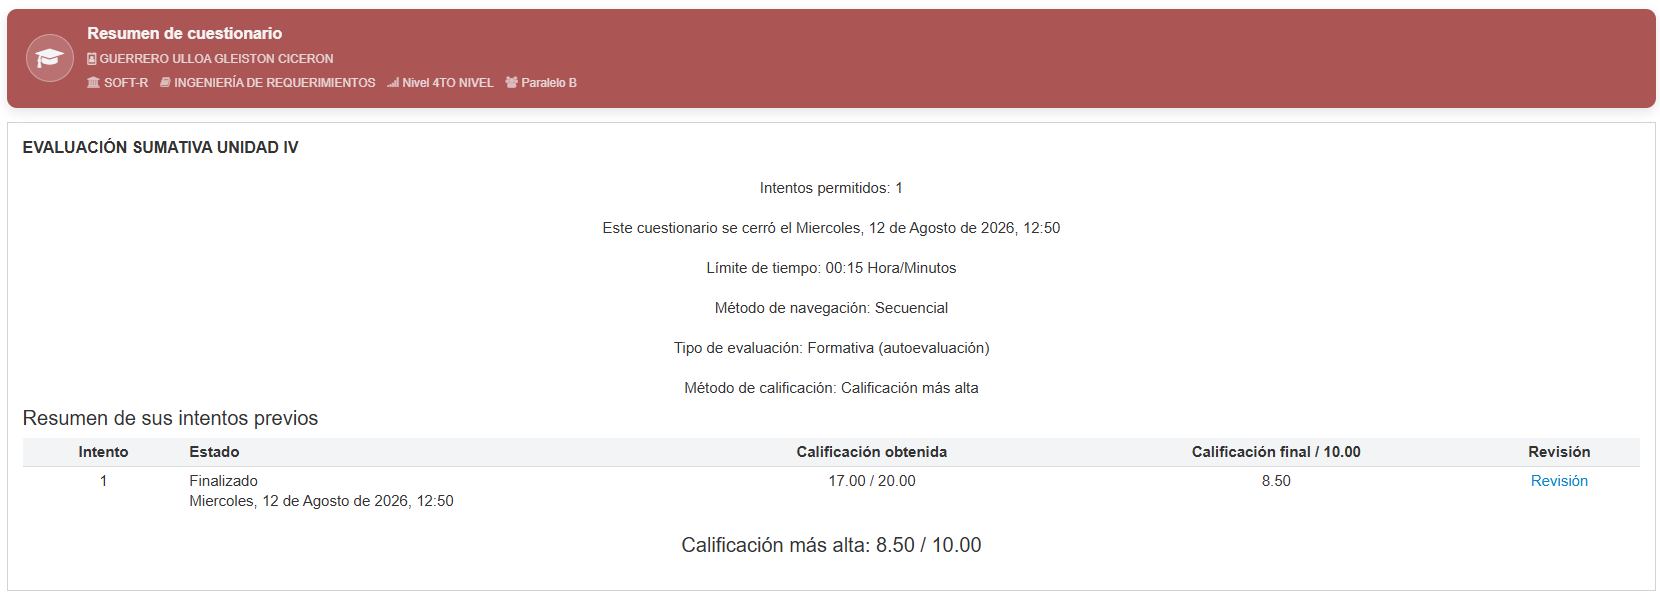
\includegraphics[width=0.95\textwidth]{figuras/Resumen_Evaluacion_LMS.png}\\[-0.05cm]
		{\small\textit{Resumen del cuestionario en el SGA.}}\\[0.25cm]
		
		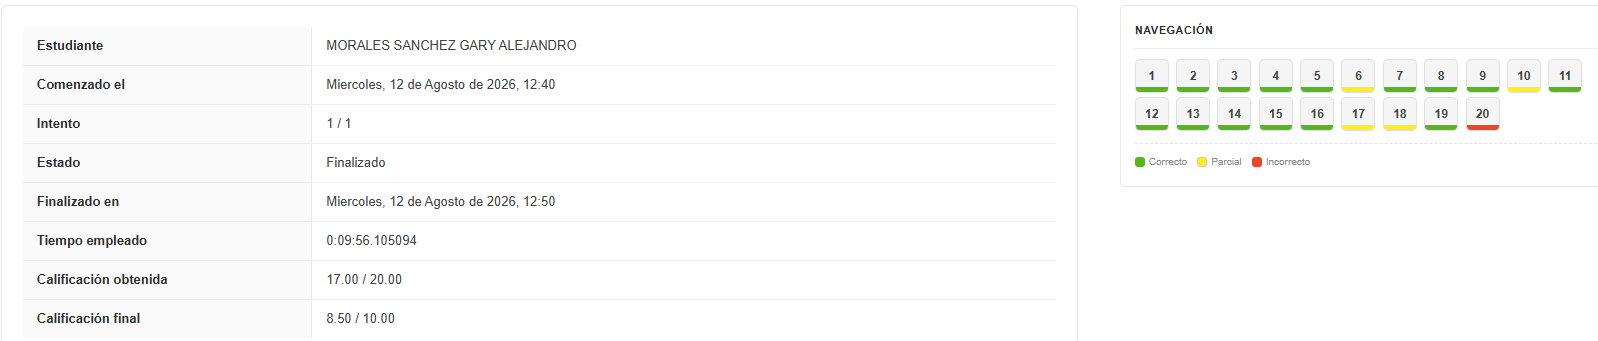
\includegraphics[width=0.95\textwidth]{figuras/Revision_intento_lms.png}\\[-0.05cm]
		{\small\textit{Evaluaci\'on/revisi\'on del intento en el SGA.}}\\[0.25cm]
		
		\vspace{16pt}
		{\small\bfseries QUEVEDO -- LOS R\'IOS -- ECUADOR \quad\textbullet\quad 2026 -- 2027 PPA}
		
	\end{titlepage}
	
	\newpage
	\sffamily
	
	% ── Portada breve / cabecera del instrumento ─────────────────────────
	\begin{center}
		{\Large\bfseries\color{darkblue} UNIVERSIDAD T\'ECNICA ESTATAL DE QUEVEDO}\\[2pt]
		{\normalsize\color{midblue} Facultad de Ciencias de la Ingenier\'ia \textbullet\ Carrera de Ingenier\'ia de Software}\\[6pt]
		{\color{gold}\rule{0.9\linewidth}{1.2pt}}\\[6pt]
		{\large\bfseries\color{darkblue} PRUEBA PR\'ACTICA --- UNIDAD IV \textbullet\ PARALELO B}\\[2pt]
		{\normalsize\color{darkblue} Validaci\'on, Gesti\'on, Herramientas y Est\'andares de Requisitos}\\[2pt]
		{\small\color{black} Asignatura: Ingenier\'ia de Requisitos (ISR-401) \quad\textbullet\quad Docente: Ing. Gleiston Guerrero, Mg.}
	\end{center}
	
	\vspace{2pt}
	\begin{center}\small
		\begin{tabularx}{\linewidth}{@{}L{2.6cm} X L{2.6cm} X@{}}
			\toprule
			\textbf{Estudiante} & Morales S\'anchez Gary Alejandro & \textbf{Fecha} & 12/08/2026\\
			\textbf{Modalidad} & Individual, en clase & \textbf{Duraci\'on} & 120 minutos \\
			\textbf{Caso} & Sistema de Reserva de Citas M\'edicas & \textbf{Ponderaci\'on} & 100 puntos (30 + 70) \\
			\bottomrule
		\end{tabularx}
	\end{center}
	
	% ── Resultado de aprendizaje ─────────────────────────────────────────
	\begin{concepto}{Resultado de aprendizaje evaluado}
		El estudiante \textbf{construye y valida} los modelos de an\'alisis (datos, funci\'on y comportamiento) de un sistema, \textbf{especifica y gestiona} sus requisitos aplicando est\'andares (\textit{ISO/IEC/IEEE} 29148:2018 e \textit{ISO/IEC} 25010:2023) y \textbf{demuestra trazabilidad, control de cambios y gesti\'on de configuraci\'on} sobre un repositorio reproducible. Esta prueba eval\'ua \emph{desempe\~no pr\'actico}: no contiene preguntas te\'oricas; se califica lo que el estudiante \emph{produce}.
	\end{concepto}
	
	% #####################################################################
	\section{Instrucciones generales y entregables}
	
	La prueba se desarrolla de forma individual durante la sesi\'on. Todo el trabajo se versiona en un \textbf{repositorio Git p\'ublico} (GitHub o GitLab) creado por el estudiante. El entregable se redacta en \textbf{LaTeX} y se compila a \textbf{PDF} dentro del propio repositorio. Al finalizar, el estudiante sube al LMS (SGA) un \textbf{PDF con car\'atula} que contiene, \textbf{en una sola l\'inea}, la \textbf{URL} del repositorio.
	
	\begin{enumerate}[leftmargin=1.4em,itemsep=1pt,topsep=2pt]
		\item \textbf{Repositorio} con: archivo principal \texttt{.tex}, archivo \texttt{referencias.bib} (si aplica), figuras, \texttt{PDF} compilado y \texttt{README.md}.
		\item \textbf{README.md} con las instrucciones exactas de compilaci\'on: compilador (\texttt{pdflatex}), orden de comandos, archivo principal y dependencias.
		\item \textbf{Car\'atula del PDF} con datos de identificaci\'on y la URL del repositorio en una sola l\'inea, m\'as la \textbf{captura del resumen} y la \textbf{captura de la evaluaci\'on} del cuestionario rendido en el SGA.
		\item Los modelos (clases, actividades, m\'aquina de estados) pueden dibujarse en \textbf{TikZ}, en una herramienta CASE (p.\,ej. Enterprise Architect / Sparx EA) o a mano y adjuntarse como imagen legible.
	\end{enumerate}
	
	% ── Criterios de piso ────────────────────────────────────────────────
	\begin{piso}{Criterios de piso --- su incumplimiento implica calificaci\'on CERO (0) en toda la prueba}
		\textbf{1. Evidencia del repositorio.} El estudiante debe subir al LMS (SGA) un documento \textbf{PDF con car\'atula} (datos de identificaci\'on) que muestre claramente, \textbf{en una sola l\'inea}, la \textbf{URL del repositorio} donde se encuentra el trabajo desarrollado. Si la URL est\'a rota, el repositorio no es accesible, o no se cumple esta directriz, la calificaci\'on es \textbf{CERO}.\\[3pt]
		\textbf{2. Reproducibilidad del PDF.} Si el PDF \textbf{no se genera} correctamente a partir del LaTeX mediante \textbf{clonaci\'on del repositorio y compilaci\'on} del archivo \texttt{.tex}, la calificaci\'on es \textbf{CERO}. Las instrucciones de compilaci\'on (compilador, orden de comandos, archivo principal, dependencias) deben estar documentadas en el archivo \texttt{README.md} del repositorio.
	\end{piso}
	
	% #####################################################################
	\section{Caso pr\'actico: Sistema de Reserva de Citas M\'edicas}
	
	Una cl\'inica requiere un m\'odulo para gestionar las reservas de citas de sus pacientes. Un \textbf{Paciente} (identificado por c\'edula, nombre y correo) puede solicitar cero o m\'as \textbf{Citas}. Cada \textbf{Cita} (identificador, fecha-hora y estado) corresponde a un \textbf{M\'edico} (c\'odigo, nombre, especialidad) sobre un \textbf{Cupo} de su agenda (fecha-hora, disponibilidad). Al agendar una cita, el sistema verifica la disponibilidad de \textbf{cupo} en la agenda del m\'edico: si hay cupo, \emph{confirma} la cita; si no, \emph{notifica la no disponibilidad} y propone otro horario. Una cita confirmada puede \emph{atenderse}, o bien \emph{cancelarse} mientras no haya sido atendida; si el paciente no se presenta, la cita se marca como \emph{no asistida}. El sistema debe registrar la cita con rapidez y proteger los datos personales del paciente.
	
	Sobre este caso, el estudiante desarrolla las diez actividades pr\'acticas siguientes. Todas las actividades usan el \emph{mismo} dominio, de modo que los modelos deben ser mutuamente consistentes.
	
	% #####################################################################
	\section{Actividades pr\'acticas (desarrollo --- 70 puntos)}
	
	\begin{tarea}{P1. Modelo de datos --- Diagrama de clases UML \hfill (8 pts)}
		Construya el \textbf{diagrama de clases UML} del dominio con al menos las clases \textsf{Paciente}, \textsf{Cita}, \textsf{M\'edico} y \textsf{Cupo} (agenda). Cada clase debe incluir sus \textbf{atributos} con tipo, al menos una \textbf{operaci\'on} pertinente y las \textbf{multiplicidades} en los extremos de cada asociaci\'on. Subraye o marque los identificadores.
	\end{tarea}
	
	\begin{figure}[H]
		\centering
		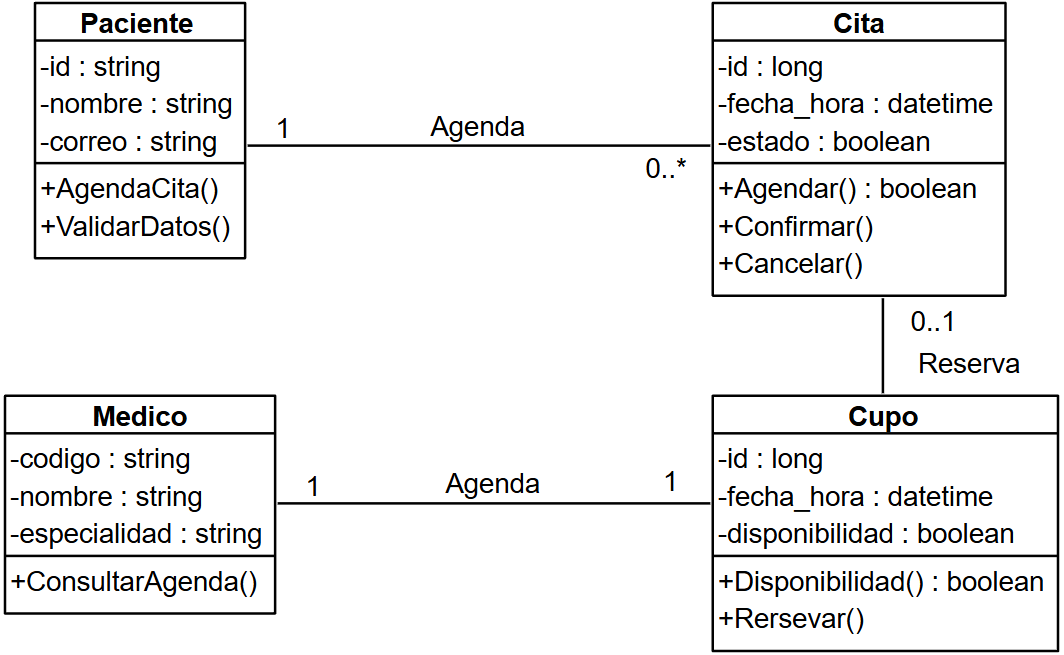
\includegraphics[width=\textwidth]{figuras/Diagramadeclases.png}
		\caption{Diagrama de clases UML --- Modelo de datos P1}
		\label{fig:clases}
	\end{figure}
	
	\begin{tarea}{P2. Modelo funcional --- Diagrama de actividades UML \hfill (8 pts)}
		Modele el proceso \textbf{``Agendar cita''} con un \textbf{diagrama de actividades UML} que incluya: nodo inicial, al menos una \textbf{decisi\'on} (\textsf{\textquestiondown cupo disponible?}), los dos caminos alternativos (\emph{confirmar} / \emph{notificar no disponibilidad}), su convergencia y el nodo final. Use carriles de responsabilidad si distingue actores.
	\end{tarea}
	
	\begin{figure}[H]
		\centering
		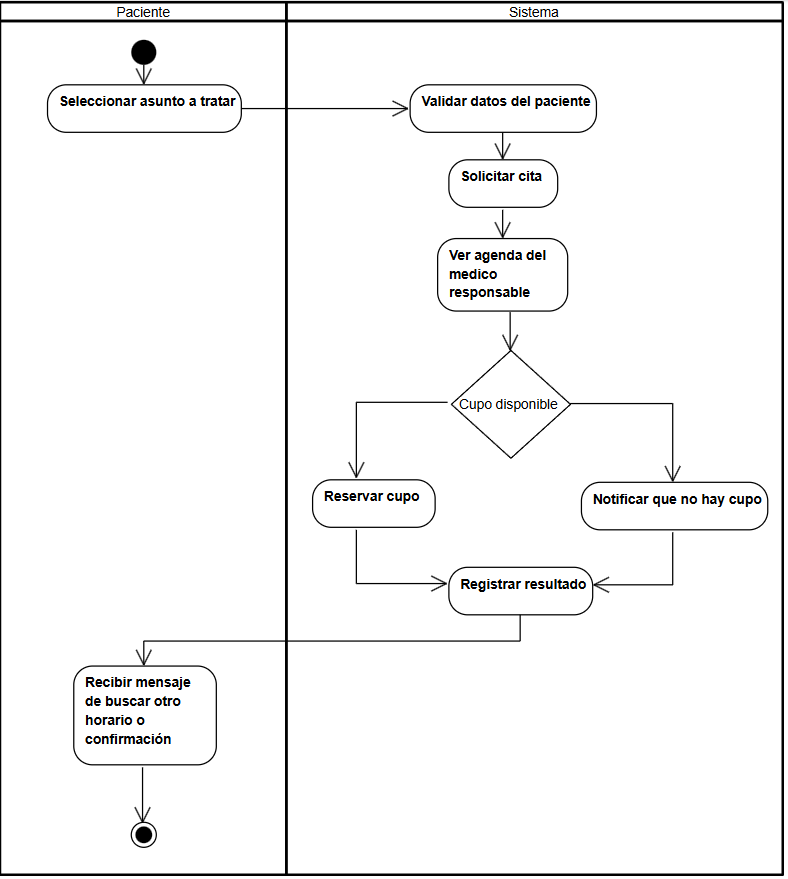
\includegraphics[height=0.78\textheight,keepaspectratio]{figuras/diagramadeactividades.png}
		\caption{Diagrama de actividades UML --- Modelo funcional P2}
		\label{fig:actividades}
	\end{figure}
	
	\begin{tarea}{P3. Modelo de comportamiento --- M\'aquina de estados UML \hfill (8 pts)}
		Elabore la \textbf{m\'aquina de estados UML} del ciclo de vida de una \textsf{Cita} (p.\,ej. \textsf{Solicitada}, \textsf{Confirmada}, \textsf{Atendida}, \textsf{Cancelada}, \textsf{No asistida}). Etiquete cada \textbf{transici\'on} con su \textbf{evento}, incluya al menos una \textbf{condici\'on de guarda} y marque el estado final de aceptaci\'on. Se valora el uso de un superestado (statechart) para factorizar la transici\'on \emph{cancelar}.
	\end{tarea}
	
	\begin{figure}[H]
		\centering
		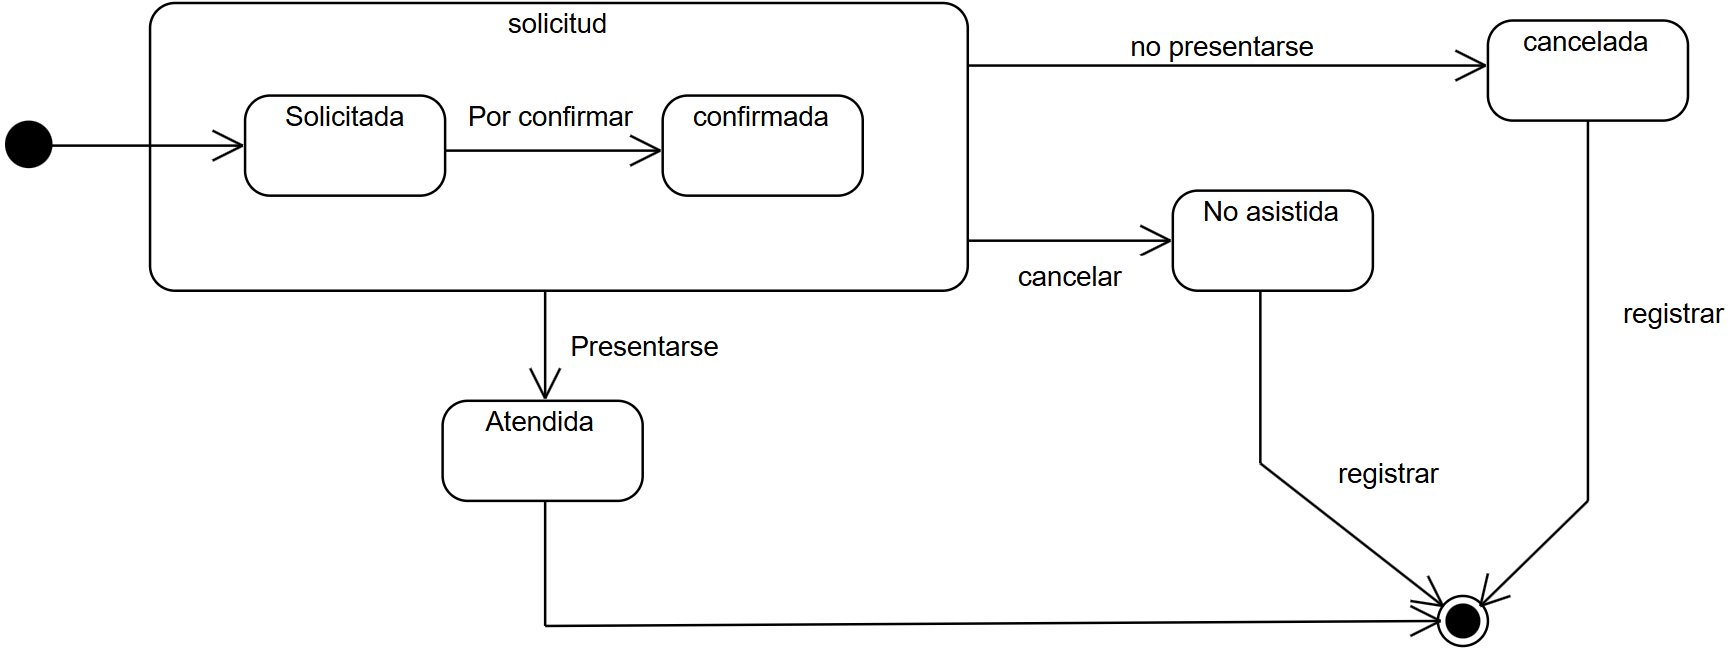
\includegraphics[width=\textwidth]{figuras/diagramamaquinadeestado.png}
		\caption{M\'aquina de estados UML --- Modelo de comportamiento P3}
		\label{fig:maquinaestado}
	\end{figure}
	
	\begin{tarea}{P4. Consistencia entre las tres perspectivas \hfill (7 pts)}
		Elabore una \textbf{tabla de verificaci\'on cruzada} que relacione cada \textbf{evento} de P3 con la \textbf{funci\'on/acci\'on} de P2 que lo realiza y con la \textbf{entidad o atributo} de P1 que modifica. \textbf{Detecte al menos una inconsistencia} entre los modelos (evento sin funci\'on, entidad sin clase, etc.), \textbf{documente} el defecto y \textbf{corrija} el modelo afectado.
	\end{tarea}
	
	\vspace{10pt}
	
	\textbf{Tabla de verificaci\'on cruzada}
	
	\begin{center}\small
		\begin{tabularx}{\linewidth}{|L{2.3cm}|X|L{3.4cm}|L{2.1cm}|}
			\hline
			\textbf{Evento (P3)} & \textbf{Funci\'on/Acci\'on (P2)} & \textbf{Entidad o atributo (P1) que modifica} & \textbf{Inconsistencia}\\
			\hline
			Solicitar & Solicitar cita & Cita.id, Cita.fecha\_hora, Cita.estado & No\\
			\hline
			Confirmar & Reservar cupo & Cita.estado & No\\
			\hline
			Rechazar & Notificar que no hay cupo & Cita.estado & No\\
			\hline
			Atender & Fuera de P2, pero est\'a indirectamente al confirmar el cupo & Cita.estado & No\\
			\hline
			No asistir & No hay funci\'on en P2 ni en P1 & Cita.estado & S\'i, DEF-01\\
			\hline
			Cancelar & No existe atributo asociado & Cita.estado & S\'i, DEF-02\\
			\hline
		\end{tabularx}
	\end{center}
	
	\vspace{10pt}
	
	\textbf{Defectos detectados y correcci\'on}
	
	\begin{center}\small
		\begin{tabularx}{\linewidth}{|L{1.8cm}|X|X|}
			\hline
			\textbf{Defecto} & \textbf{Descripci\'on} & \textbf{Correcci\'on}\\
			\hline
			DEF-01 & El evento no tiene funci\'on asociada, tampoco operaciones. & Se incorpora una funci\'on y una operaci\'on que definan qu\'e ocurre si el paciente no asiste a la cita.\\
			\hline
			DEF-02 & No existe un atributo que soporte la cancelaci\'on en la clase. & Se modifica el atributo \textsf{estado} de la clase \textsf{Cita} para que admita m\'as valores, como \emph{cancelada}, adem\'as de \emph{atendida} o \emph{no asistida}, en lugar de un valor booleano.\\
			\hline
		\end{tabularx}
	\end{center}
	
	\newpage
	
	\begin{tarea}{P5. Especificaci\'on de requisitos con esquema de atributos \hfill (10 pts)}
		Redacte \textbf{4 requisitos}: \textbf{2 funcionales} y \textbf{2 no funcionales}. Cada requisito no funcional debe \textbf{nombrar una caracter\'istica de \textit{ISO/IEC} 25010:2023} (p.\,ej. Eficiencia de desempe\~no, Seguridad), fijar una \textbf{m\'etrica} y un \textbf{umbral} (p.\,ej. ``agendar la cita en $<$ 3 s''). Para cada requisito complete un \textbf{esquema de atributos}: identificador, prioridad, estado, fuente, estabilidad, versi\'on y m\'etodo de verificaci\'on.
	\end{tarea}
	
	\vspace{10pt}
	
	\textbf{Requisitos especificados}
	
	\begin{center}\small
		\begin{tabularx}{\linewidth}{|L{1.5cm}|L{2.4cm}|X|}
			\hline
			\textbf{ID} & \textbf{Tipo} & \textbf{Descripci\'on}\\
			\hline
			RF-01 & Funcional & El sistema deber\'a verificar la disponibilidad de un cupo para confirmar la cita o, en caso contrario, notificar y proponer otro horario.\\
			\hline
			RF-02 & Funcional & El sistema deber\'a permitir cancelar una cita mientras no haya sido atendida.\\
			\hline
			RNF-01 & No funcional & Eficiencia: el sistema deber\'a responder en menos de 3 segundos al agendar una cita.\\
			\hline
			RNF-02 & No funcional & Seguridad: el sistema deber\'a cifrar los datos personales del paciente.\\
			\hline
		\end{tabularx}
	\end{center}
	
	\vspace{10pt}
	
	\textbf{M\'etricas y umbrales de los requisitos no funcionales}
	
	\begin{center}\small
		\begin{tabularx}{\linewidth}{|L{1.5cm}|L{3.0cm}|X|L{3.2cm}|}
			\hline
			\textbf{Tipo} & \textbf{Norma ISO/IEC 25010:2023} & \textbf{M\'etrica} & \textbf{Umbral}\\
			\hline
			RNF-01 & Eficiencia de desempe\~no & Tiempo de respuesta, percentil 95, con 100 usuarios/pacientes concurrentes & P95 $<$ 3 segundos\\
			\hline
			RNF-02 & Seguridad & Porcentaje de campos cifrados del paciente & 100\,\% de los datos de pacientes/usuarios cifrados\\
			\hline
		\end{tabularx}
	\end{center}
	
	\vspace{10pt}
	
	\textbf{Esquema de atributos de los requisitos}
	
	\begin{center}\footnotesize
		\begin{tabularx}{\linewidth}{|L{1.2cm}|L{1.4cm}|L{1.6cm}|X|L{1.6cm}|L{1.2cm}|L{2.2cm}|}
			\hline
			\textbf{ID} & \textbf{Prioridad} & \textbf{Estado} & \textbf{Fuente} & \textbf{Estabilidad} & \textbf{Versi\'on} & \textbf{M\'etodo de verificaci\'on}\\
			\hline
			RF-01 & Alta & Aprobado & Enunciado del caso: ``el sistema verifica la disponibilidad de cupo en la agenda del m\'edico'' (l\'ineas 4, 5 y 6) & Alta & v1.0 & Prueba\\
			\hline
			RF-02 & Media & Aprobado & Enunciado del caso, l\'ineas 6 y 7 & Media & v1.0 & Prueba\\
			\hline
			RNF-01 & Alta & Propuesto & Enunciado del caso, l\'inea 8 & Media & v1.0 & Prueba de carga\\
			\hline
			RNF-02 & Alta & Propuesto & Enunciado del caso, l\'inea 5 & Alta & v1.0 & Inspecci\'on de configuraci\'on\\
			\hline
		\end{tabularx}
	\end{center}
	
	\vspace{10pt}
	
	\begin{tarea}{P6. Priorizaci\'on MoSCoW \hfill (5 pts)}
		Clasifique los 4 requisitos de P5 en las categor\'ias \textbf{MoSCoW} (\textit{Must / Should / Could / Won't have this time}) y \textbf{justifique} brevemente cada asignaci\'on en funci\'on del valor y la viabilidad. Al menos un requisito debe ser \textit{Must have}.
	\end{tarea}
	
	\vspace{10pt}
	
	\begin{center}\small
		\begin{tabularx}{\linewidth}{|L{1.6cm}|L{2.4cm}|X|}
			\hline
			\textbf{ID} & \textbf{MoSCoW} & \textbf{Justificaci\'on}\\
			\hline
			RF-01 & Must have & Sin verificaci\'on de cupo y confirmaci\'on no existe la reserva de cita; es la funci\'on n\'ucleo del sistema.\\
			\hline
			RF-02 & Should have & La cl\'inica puede operar temporalmente sin la cancelaci\'on en l\'inea, aunque su ausencia degrada el servicio.\\
			\hline
			RNF-01 & Could have & Un tiempo de respuesta mayor no impide agendar ni solicitar una cita, por lo que puede diferirse.\\
			\hline
			RNF-02 & Must have & La cl\'inica podr\'ia ser sancionada por el tratamiento indebido de los datos personales del paciente.\\
			\hline
		\end{tabularx}
	\end{center}
	
	\newpage
	
	\begin{tarea}{P7. Validaci\'on por inspecci\'on (lista de comprobaci\'on 29148) \hfill (8 pts)}
		Aplique a los requisitos de P5 una \textbf{lista de comprobaci\'on} derivada de las propiedades de \textit{ISO/IEC/IEEE} 29148 (no ambiguo, completo, singular, verificable, factible). \textbf{Registre los defectos detectados sin corregirlos en el momento} (separar identificaci\'on de correcci\'on) y, en un segundo paso, presente el \textbf{retrabajo} con los requisitos corregidos.
	\end{tarea}
	
	\vspace{10pt}
	
	\textbf{Paso 1 --- Lista de comprobaci\'on e identificaci\'on de defectos (sin corregir)}
	
	\begin{center}\footnotesize
		\begin{tabularx}{\linewidth}{|L{1.2cm}|L{1.5cm}|L{1.3cm}|L{1.3cm}|L{1.5cm}|L{1.2cm}|X|}
			\hline
			\textbf{ID} & \textbf{No ambiguo} & \textbf{Completo} & \textbf{Singular} & \textbf{Verificable} & \textbf{Factible} & \textbf{Defectos registrados}\\
			\hline
			RF-01 & No cumple & Cumple & No cumple & Cumple & Cumple & DF-01: no es singular, porque a\~nade acciones adicionales como notificar. DF-02: es ambiguo, no especifica los detalles de la elecci\'on del horario.\\
			\hline
			RF-02 & Cumple & No cumple & Cumple & Cumple & Cumple & DF-03: no es completo, no especifica qui\'en debe cancelar ni con cu\'anto tiempo de anticipaci\'on.\\
			\hline
			RNF-01 & No cumple & No cumple & Cumple & No cumple & Cumple & DF-04: no es verificable, porque no fija un percentil ni una carga concreta al exigir una respuesta menor a 3 segundos.\\
			\hline
			RNF-02 & No cumple & Cumple & Cumple & No cumple & Cumple & DF-05: no es verificable, ya que no especifica el tipo de cifrado.\\
			\hline
		\end{tabularx}
	\end{center}
	
	\vspace{10pt}
	
	\textbf{Paso 2 --- Retrabajo de los requisitos corregidos}
	
	\begin{center}\small
		\begin{tabularx}{\linewidth}{|L{1.8cm}|L{1.5cm}|X|}
			\hline
			\textbf{Requisito} & \textbf{Defecto} & \textbf{Correcci\'on}\\
			\hline
			RF-01.1 & DF-01 & El sistema deber\'a verificar la disponibilidad de un cupo en la agenda del m\'edico para la fecha y hora solicitadas.\\
			\hline
			RF-01.2 & DF-02 & El sistema deber\'a notificar al paciente cuando el cupo no est\'e disponible y proponer 2 cupos libres del mismo m\'edico, ordenados por fecha y hora.\\
			\hline
			RF-02 & DF-03 & El sistema deber\'a permitir cancelar una cita hasta un d\'ia antes de la fecha y hora seleccionadas.\\
			\hline
			RNF-01 & DF-04 & El sistema responder en menos de 3 segundos al agendar una cita, seg\'un el percentil 95, con 100 usuarios solicitando citas de forma concurrente.\\
			\hline
			RNF-02 & DF-05 & El sistema deber\'a almacenar cifrados con AES-256 la c\'edula, el nombre y el correo del paciente.\\
			\hline
		\end{tabularx}
	\end{center}
	
	\vspace{10pt}
	
	\begin{tarea}{P8. Pruebas de aceptaci\'on trazadas \hfill (6 pts)}
		Defina \textbf{una prueba de aceptaci\'on por requisito} (4 en total), indicando su \textbf{tipo} (funcional, no funcional o regresi\'on), sus \textbf{entradas}, el \textbf{criterio de \'exito} y el \textbf{requisito al que traza}. Cada prueba debe enlazar expl\'icitamente con al menos un requisito de P5.
	\end{tarea}
	
	% TODO: contenido no incluido en el documento fuente. Completar antes de entregar.
	
	\vspace{10pt}
	
	\begin{tarea}{P9. Matriz de trazabilidad \hfill (6 pts)}
		Construya la \textbf{matriz de trazabilidad} que cruce los requisitos con: su \textbf{fuente} (traza hacia atr\'as) y sus \textbf{modelos y pruebas de aceptaci\'on} (traza hacia adelante). Marque tambi\'en al menos una dependencia \textbf{horizontal} entre requisitos e \textbf{identifique} cualquier requisito hu\'erfano (sin prueba o sin modelo asociado).
	\end{tarea}
	
	% TODO: contenido no incluido en el documento fuente. Completar antes de entregar.
	
	\vspace{10pt}
	
	\begin{tarea}{P10. Gesti\'on del cambio y l\'inea base \hfill (4 pts)}
		Simule \textbf{una solicitud de cambio} sobre un requisito: reg\'istrela, \textbf{analice su impacto} usando la matriz de P9, indique la \textbf{decisi\'on del CCB} (aprobada/rechazada/diferida) y \textbf{actualice la versi\'on} del requisito. Finalmente, declare una \textbf{l\'inea base}: liste la \textbf{configuraci\'on} (versiones coherentes de ERS, modelos, matriz y pruebas) que se congela.
	\end{tarea}
	
	% TODO: contenido no incluido en el documento fuente. Completar antes de entregar.
	
	% #####################################################################
	\section{R\'ubrica de evaluaci\'on}
	
	La calificaci\'on total es de \textbf{100 puntos}, distribuidos en \textbf{30\%} para el cuestionario rendido en el LMS (SGA) y \textbf{70\%} para el desarrollo de la prueba pr\'actica. Los \textbf{criterios de piso} de la Secci\'on~1 se aplican \emph{antes} de sumar puntos: si alguno se incumple, la calificaci\'on final es \textbf{CERO}, con independencia de los puntos logrados en cada criterio.
	
	\begin{concepto}{Escala de niveles de logro (se aplica a cada criterio de la prueba pr\'actica)}
		\textbf{Logrado (100\% del peso):} el producto cumple \'integramente lo solicitado, es correcto y consistente. \quad \textbf{Parcial (60\%):} cumple lo esencial pero con omisiones o errores menores. \quad \textbf{Insuficiente (30\%):} entrega incompleta o con errores conceptuales relevantes. \quad \textbf{No entregado (0\%):} ausente o no evaluable.
	\end{concepto}
	
	% ── Componente SGA 30% ──
	\begin{table}[htbp]
		\centering
		\caption{Componente 1 --- Cuestionario en el LMS (SGA). Peso: 30 puntos.}
		\small
		\begin{tabularx}{\linewidth}{@{}L{4.6cm} C{1.6cm} X@{}}
			\toprule
			\hd{Criterio} & \hd{Peso} & \hd{Evidencia requerida}\\
			\midrule
			Nota obtenida en el cuestionario del SGA & 20 pts & Puntaje autocalificado por el LMS, proporcional al porcentaje de aciertos.\\
			\rowcolor{rowgray}
			Captura del \emph{resumen} del cuestionario en la car\'atula & 5 pts & Imagen legible del resumen de resultados incrustada en la portada del PDF.\\
			Captura de la \emph{evaluaci\'on} (intento) en la car\'atula & 5 pts & Imagen legible del intento/evaluaci\'on incrustada en la portada del PDF.\\
			\bottomrule
		\end{tabularx}
	\end{table}
	
	% ── Componente practica 70% (landscape) ──
	\begin{landscape}
		\begin{table}[htbp]
			\centering
			\caption{Componente 2 --- Desarrollo de la prueba pr\'actica. Peso: 70 puntos. (Logrado 100\% / Parcial 60\% / Insuficiente 30\% / No entregado 0\% del peso indicado.)}
			\scriptsize
			\renewcommand{\arraystretch}{1.2}
			\begin{tabularx}{\linewidth}{@{}L{3.0cm} C{0.9cm} X X X@{}}
				\toprule
				\hd{Criterio (tarea)} & \hd{Peso} & \hd{Logrado (100\%)} & \hd{Parcial (60\%)} & \hd{Insuficiente (30\%)}\\
				\midrule
				P1. Diagrama de clases UML & 8 & Clases, atributos tipados, operaciones y multiplicidades correctas y coherentes con el caso. & Faltan operaciones o alguna multiplicidad; estructura b\'asica correcta. & Clases incompletas o sin multiplicidades; errores de modelado.\\
				\rowcolor{rowgray}
				P2. Diagrama de actividades UML & 8 & Decisi\'on de \textit{cupo}, ambos caminos, convergencia y nodo final bien modelados. & Flujo correcto pero sin decisi\'on o sin convergencia expl\'icita. & Secuencia lineal sin l\'ogica de control del caso.\\
				P3. M\'aquina de estados UML & 8 & Estados, eventos, guarda y estado final; superestado bien usado. & Estados y eventos correctos, sin guarda o sin estado final. & Estados incompletos o transiciones sin evento.\\
				\rowcolor{rowgray}
				P4. Consistencia entre perspectivas & 7 & Tabla cruzada completa; inconsistencia detectada, documentada y corregida. & Tabla parcial o inconsistencia detectada pero no corregida. & Tabla ausente o sin an\'alisis de correspondencia.\\
				P5. Requisitos con esquema de atributos & 10 & 4 requisitos (2 F, 2 NF) con caracter\'istica 25010, m\'etrica, umbral y atributos completos. & Requisitos correctos con atributos incompletos o sin umbral. & Requisitos ambiguos o sin esquema de atributos.\\
				\rowcolor{rowgray}
				P6. Priorizaci\'on MoSCoW & 5 & Cuatro requisitos clasificados y justificados; al menos un \textit{Must}. & Clasificaci\'on correcta con justificaci\'on d\'ebil. & Clasificaci\'on sin justificar o mal aplicada.\\
				P7. Inspecci\'on 29148 (defectos + retrabajo) & 8 & Checklist aplicada; defectos registrados sin corregir y retrabajo presentado. & Defectos detectados sin retrabajo, o correcci\'on mezclada con detecci\'on. & Sin checklist o sin evidencia de defectos.\\
				\rowcolor{rowgray}
				P8. Pruebas de aceptaci\'on trazadas & 6 & 4 pruebas con tipo, entradas, criterio de \'exito y traza al requisito. & Pruebas sin tipo o sin criterio de \'exito claro. & Pruebas sin traza a requisitos.\\
				P9. Matriz de trazabilidad & 6 & Trazas hacia atr\'as, adelante y horizontal; hu\'erfanos identificados. & Matriz parcial (solo un sentido de traza). & Matriz ausente o sin correspondencias reales.\\
				\rowcolor{rowgray}
				P10. Gesti\'on del cambio y l\'inea base & 4 & Solicitud, impacto, decisi\'on CCB, versi\'on y configuraci\'on/baseline declarada. & Cambio registrado sin impacto o sin baseline. & Sin proceso de cambio ni l\'inea base.\\
				\midrule
				\hg{Total del componente pr\'actico} & \hg{70} & \multicolumn{3}{c}{\cellcolor{lightgray}\small\color{darkblue} Suma de puntos logrados por nivel en cada criterio.}\\
				\bottomrule
			\end{tabularx}
		\end{table}
	\end{landscape}
	
	\begin{table}[htbp]
		\centering
		\caption{Resumen de ponderaci\'on final.}
		\small
		\begin{tabularx}{\linewidth}{@{}X C{2.4cm} C{3.0cm}@{}}
			\toprule
			\hd{Componente} & \hd{Peso} & \hd{Condici\'on}\\
			\midrule
			Cuestionario en el LMS (SGA) + capturas en car\'atula & 30 pts & Sujeto a criterios de piso\\
			\rowcolor{rowgray}
			Desarrollo de la prueba pr\'actica (P1--P10) & 70 pts & Sujeto a criterios de piso\\
			\midrule
			\hg{Total} & \hg{100 pts} & \hg{CERO si se incumple un criterio de piso}\\
			\bottomrule
		\end{tabularx}
	\end{table}
	
	% #####################################################################
	\section{Marco normativo de referencia}
	
	Esta prueba operacionaliza las propiedades de calidad de la norma \textit{ISO/IEC/IEEE} 29148:2018 \citep{iso29148_2018} y el modelo de calidad de producto \textit{ISO/IEC} 25010:2023 \citep{iso25010_2023}, junto con las t\'ecnicas de validaci\'on y gesti\'on descritas por Pohl \citep{pohl_2010}, la inspecci\'on formal de Fagan \citep{fagan_1976} y las buenas pr\'acticas recogidas en la gu\'ia SWEBOK v4 \citep{swebok_v4_2024}. Las notaciones de modelado siguen la especificaci\'on \textit{OMG UML} 2.5.1 \citep{omg_uml_2017}.
	
	\vspace{4pt}
	\renewcommand{\refname}{Referencias}
	\bibliographystyle{plainnat}
	\bibliography{referencias}
	
	% ── Anexo: revision del intento en el SGA (paginas a sangre) ──────────
	\newgeometry{margin=0pt}
	\newpage
	\thispagestyle{empty}
	\noindent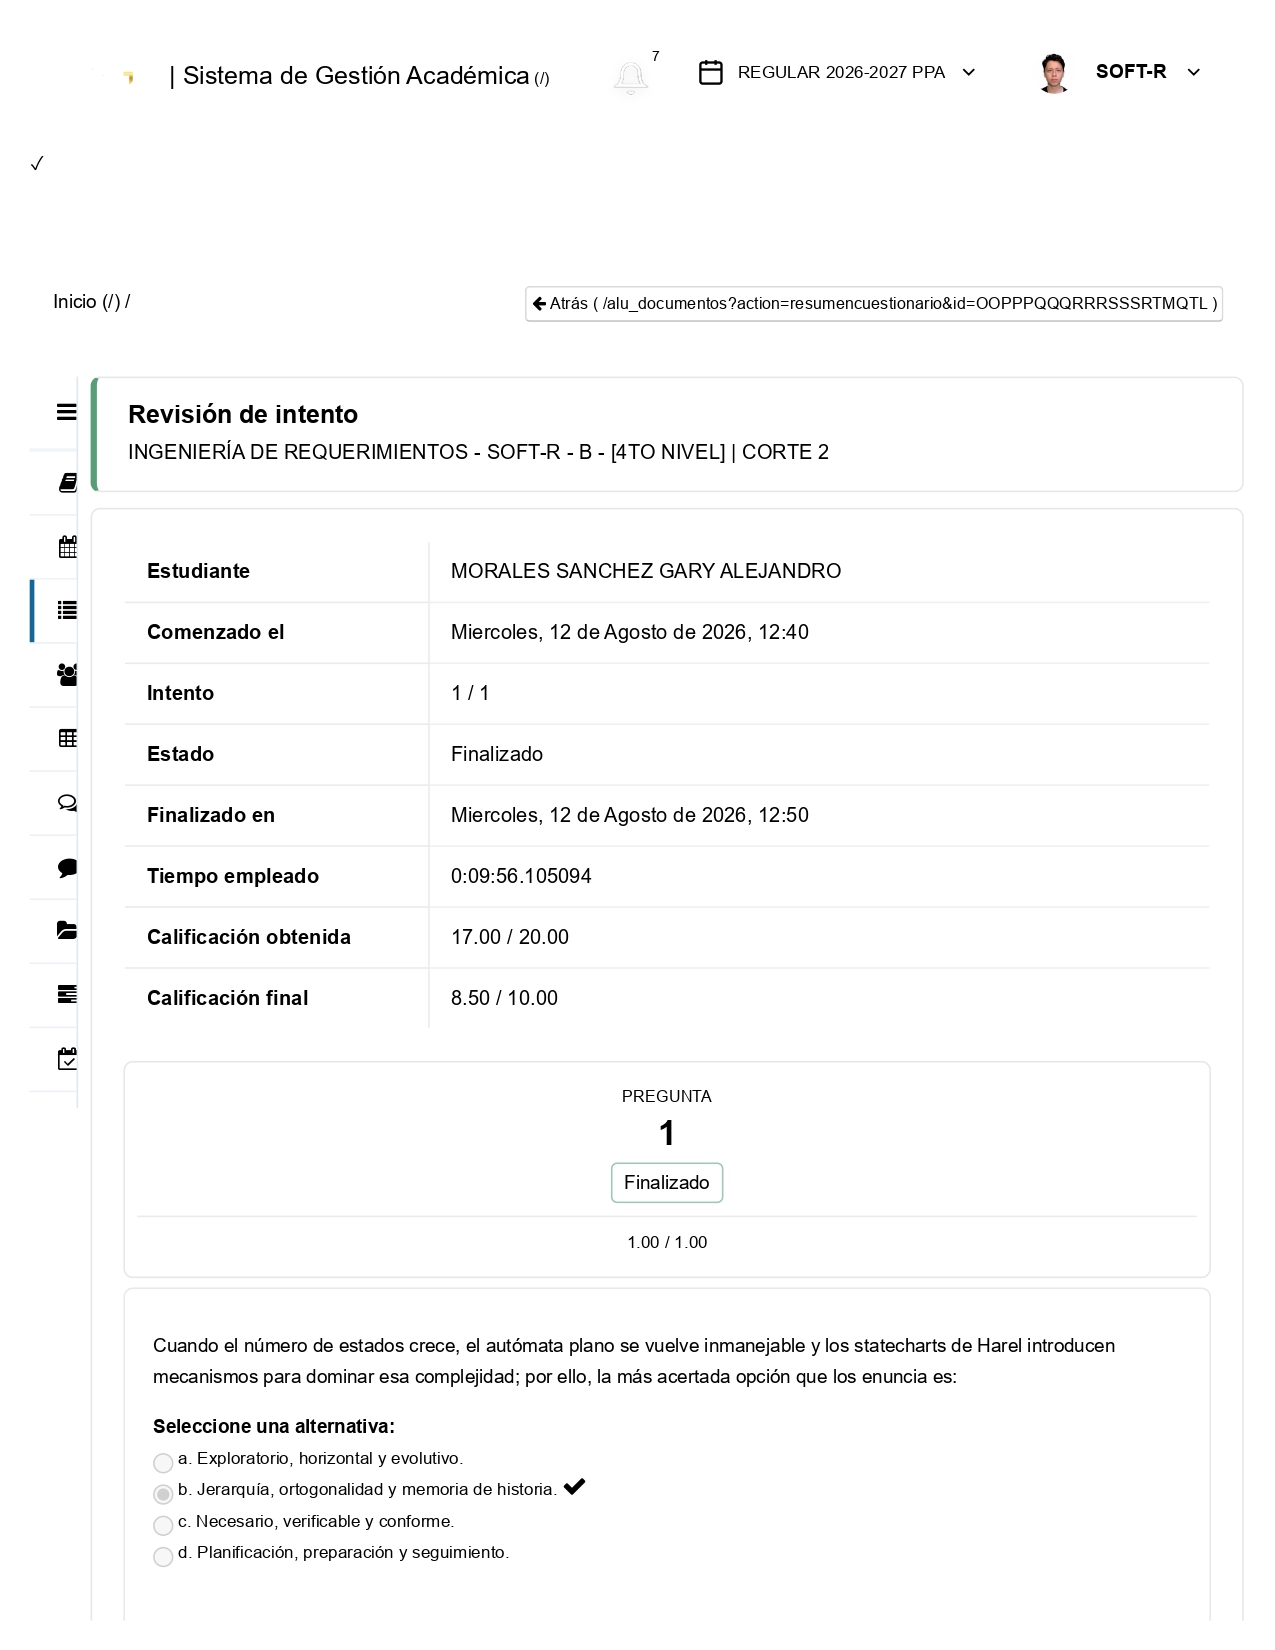
\includegraphics[width=\paperwidth,height=\paperheight,keepaspectratio]{figuras/revision_pg-1.jpg}\par
	\newpage
	\thispagestyle{empty}
	\noindent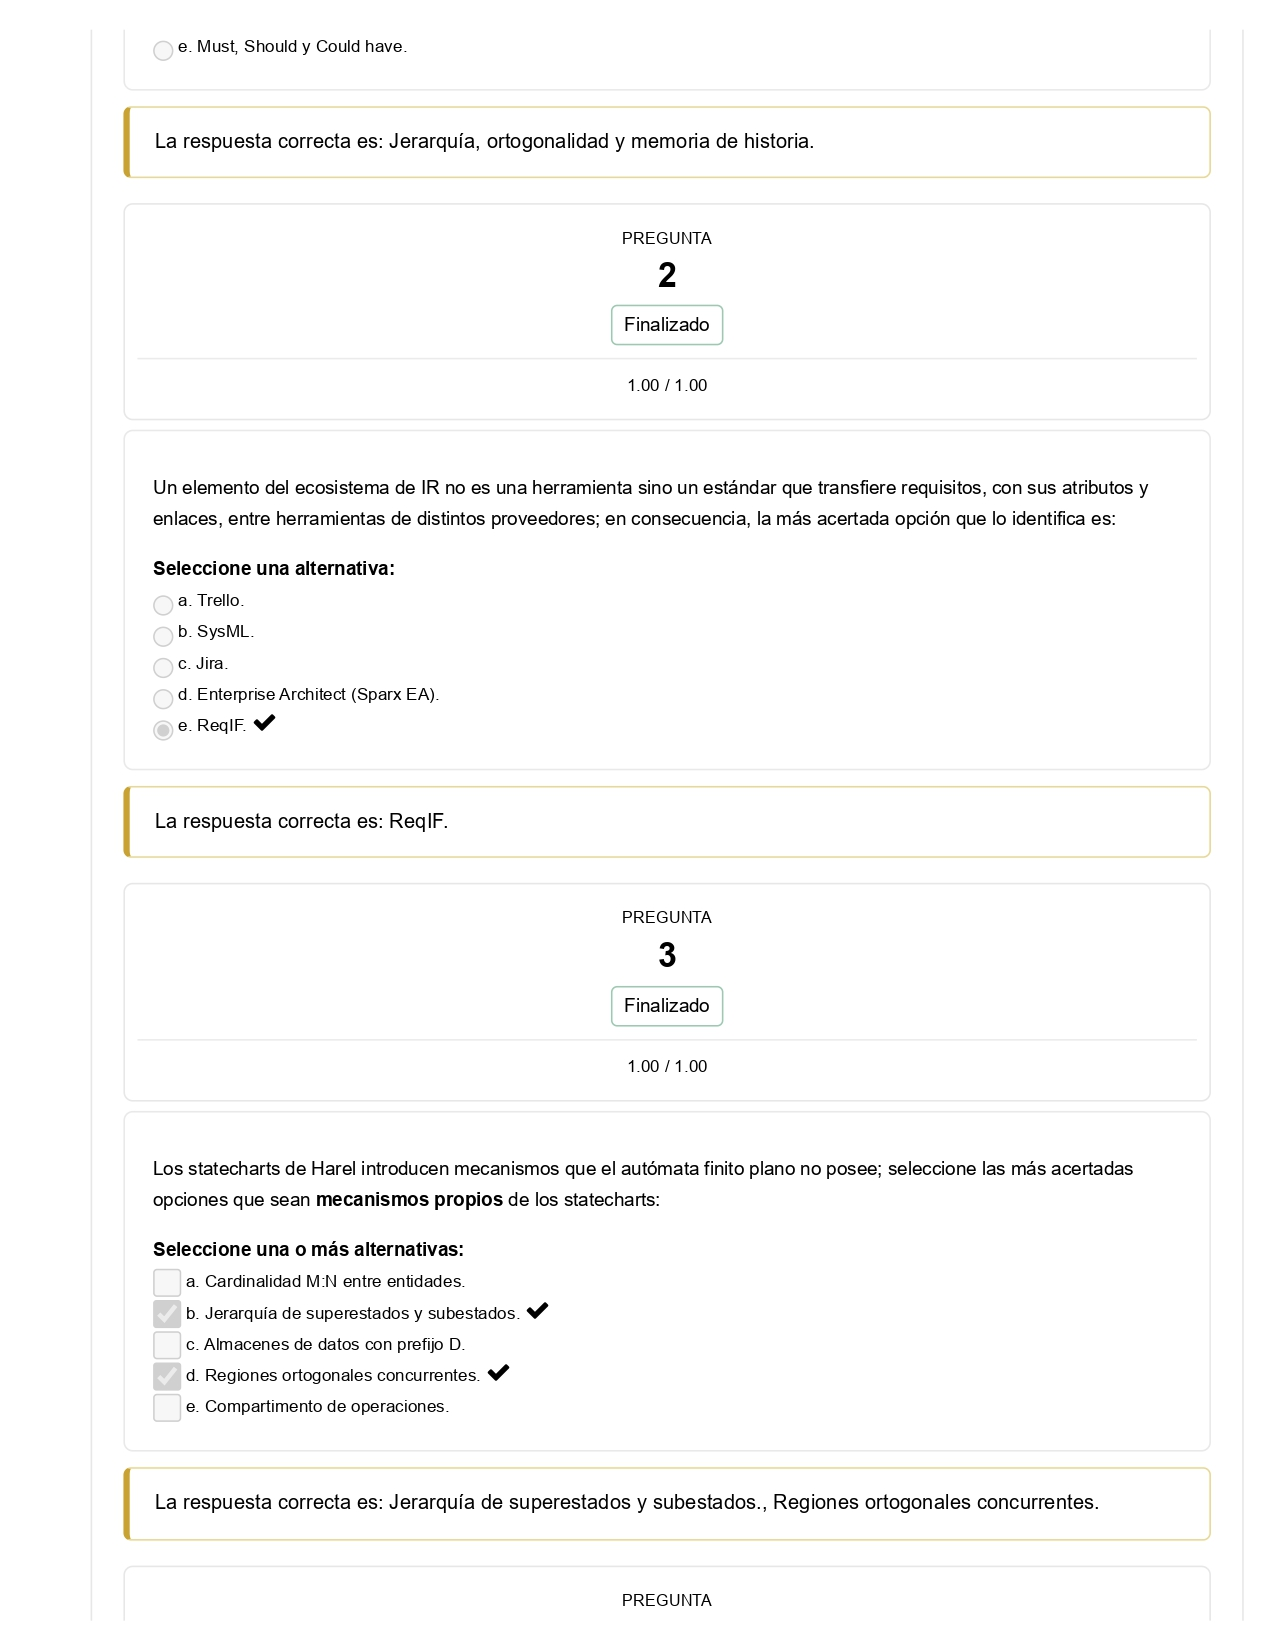
\includegraphics[width=\paperwidth,height=\paperheight,keepaspectratio]{figuras/revision_pg-2.jpg}\par
	\newpage
	\thispagestyle{empty}
	\noindent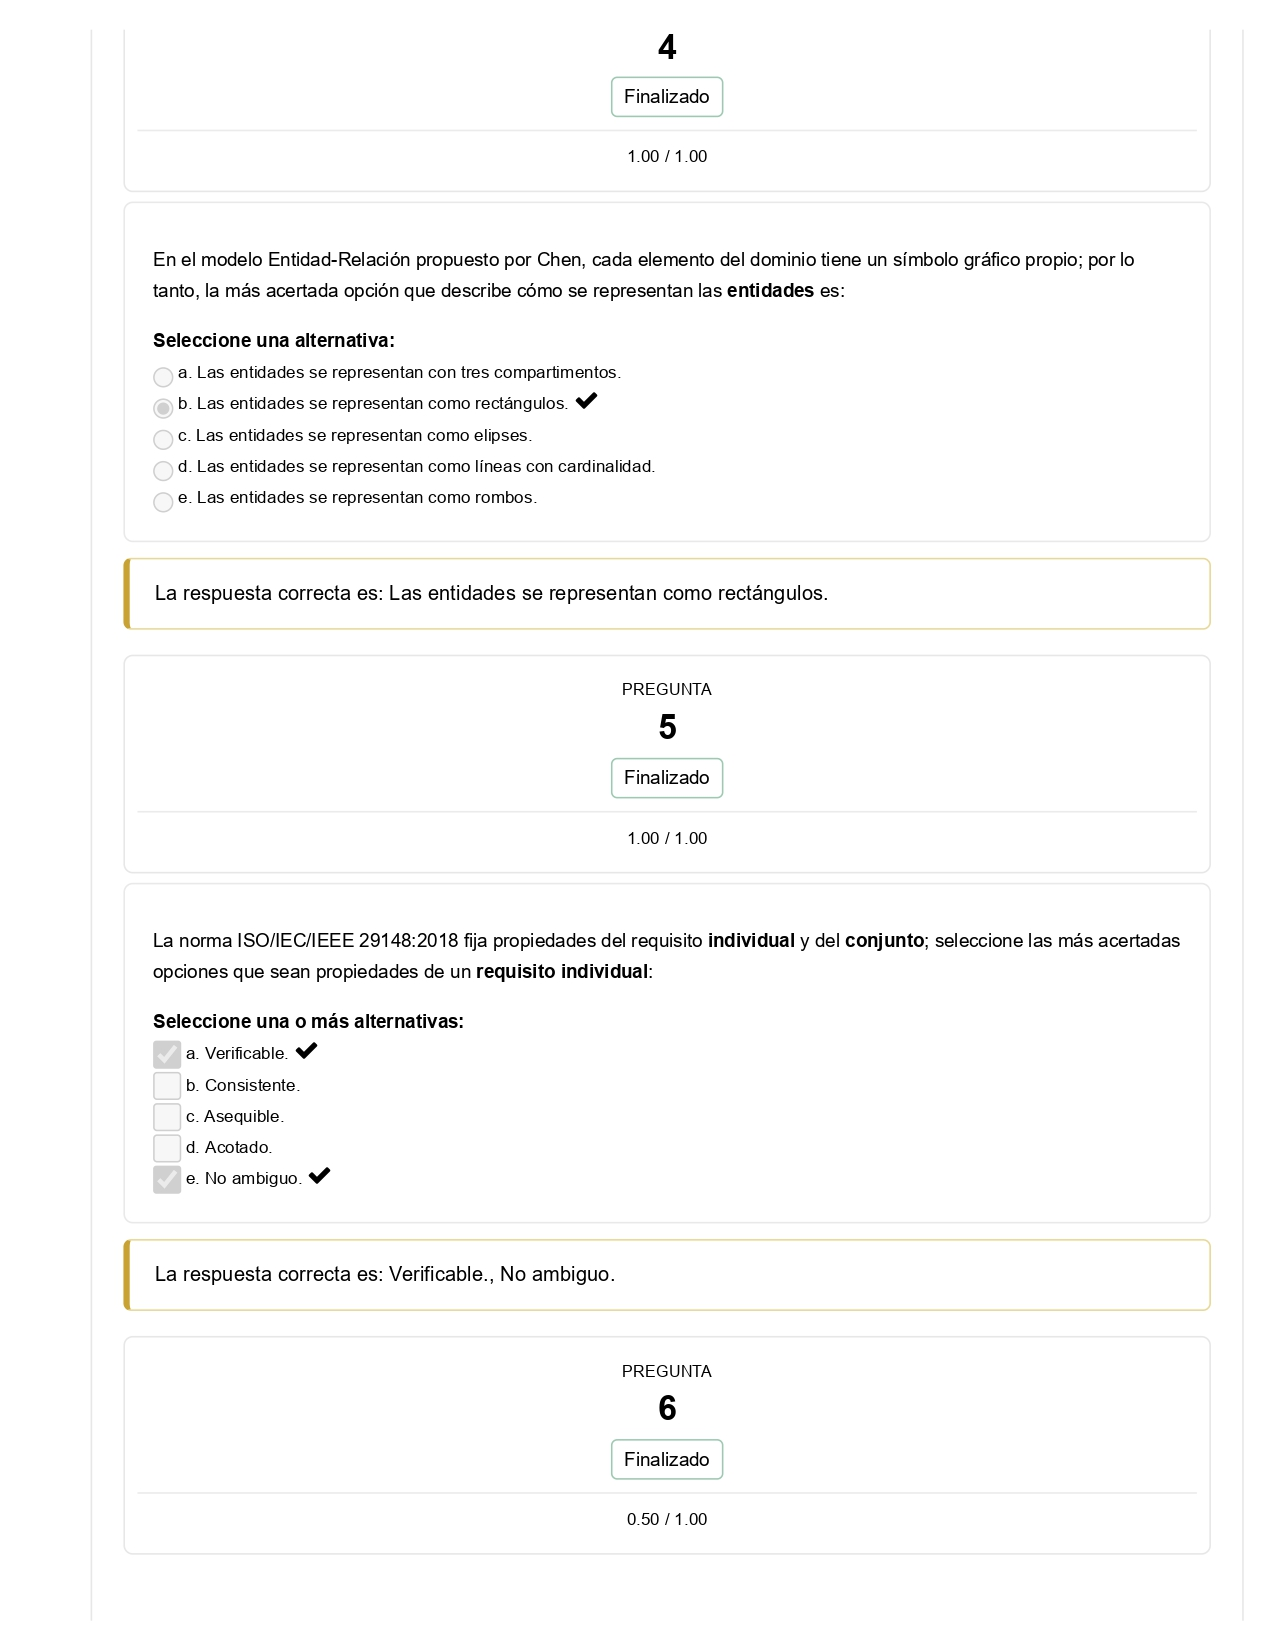
\includegraphics[width=\paperwidth,height=\paperheight,keepaspectratio]{figuras/revision_pg-3.jpg}\par
	\newpage
	\thispagestyle{empty}
	\noindent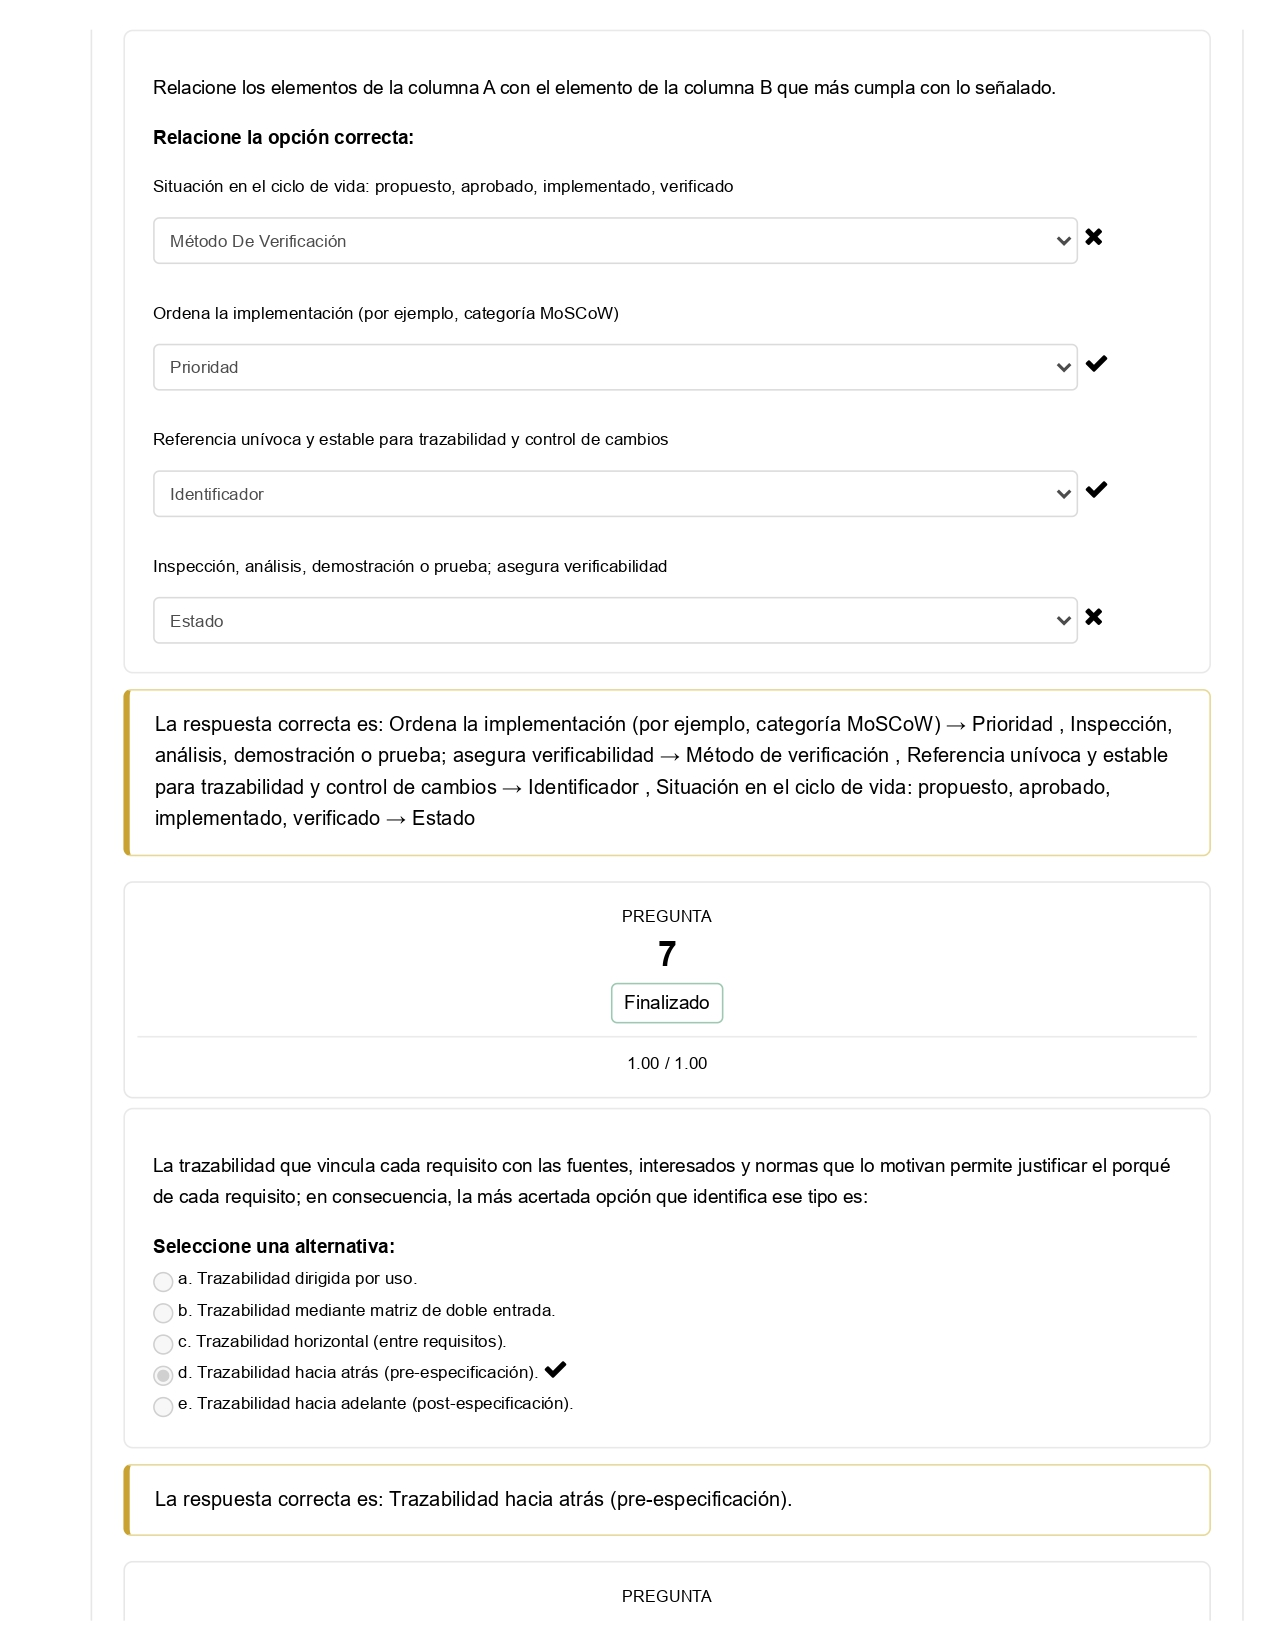
\includegraphics[width=\paperwidth,height=\paperheight,keepaspectratio]{figuras/revision_pg-4.jpg}\par
	\newpage
	\thispagestyle{empty}
	\noindent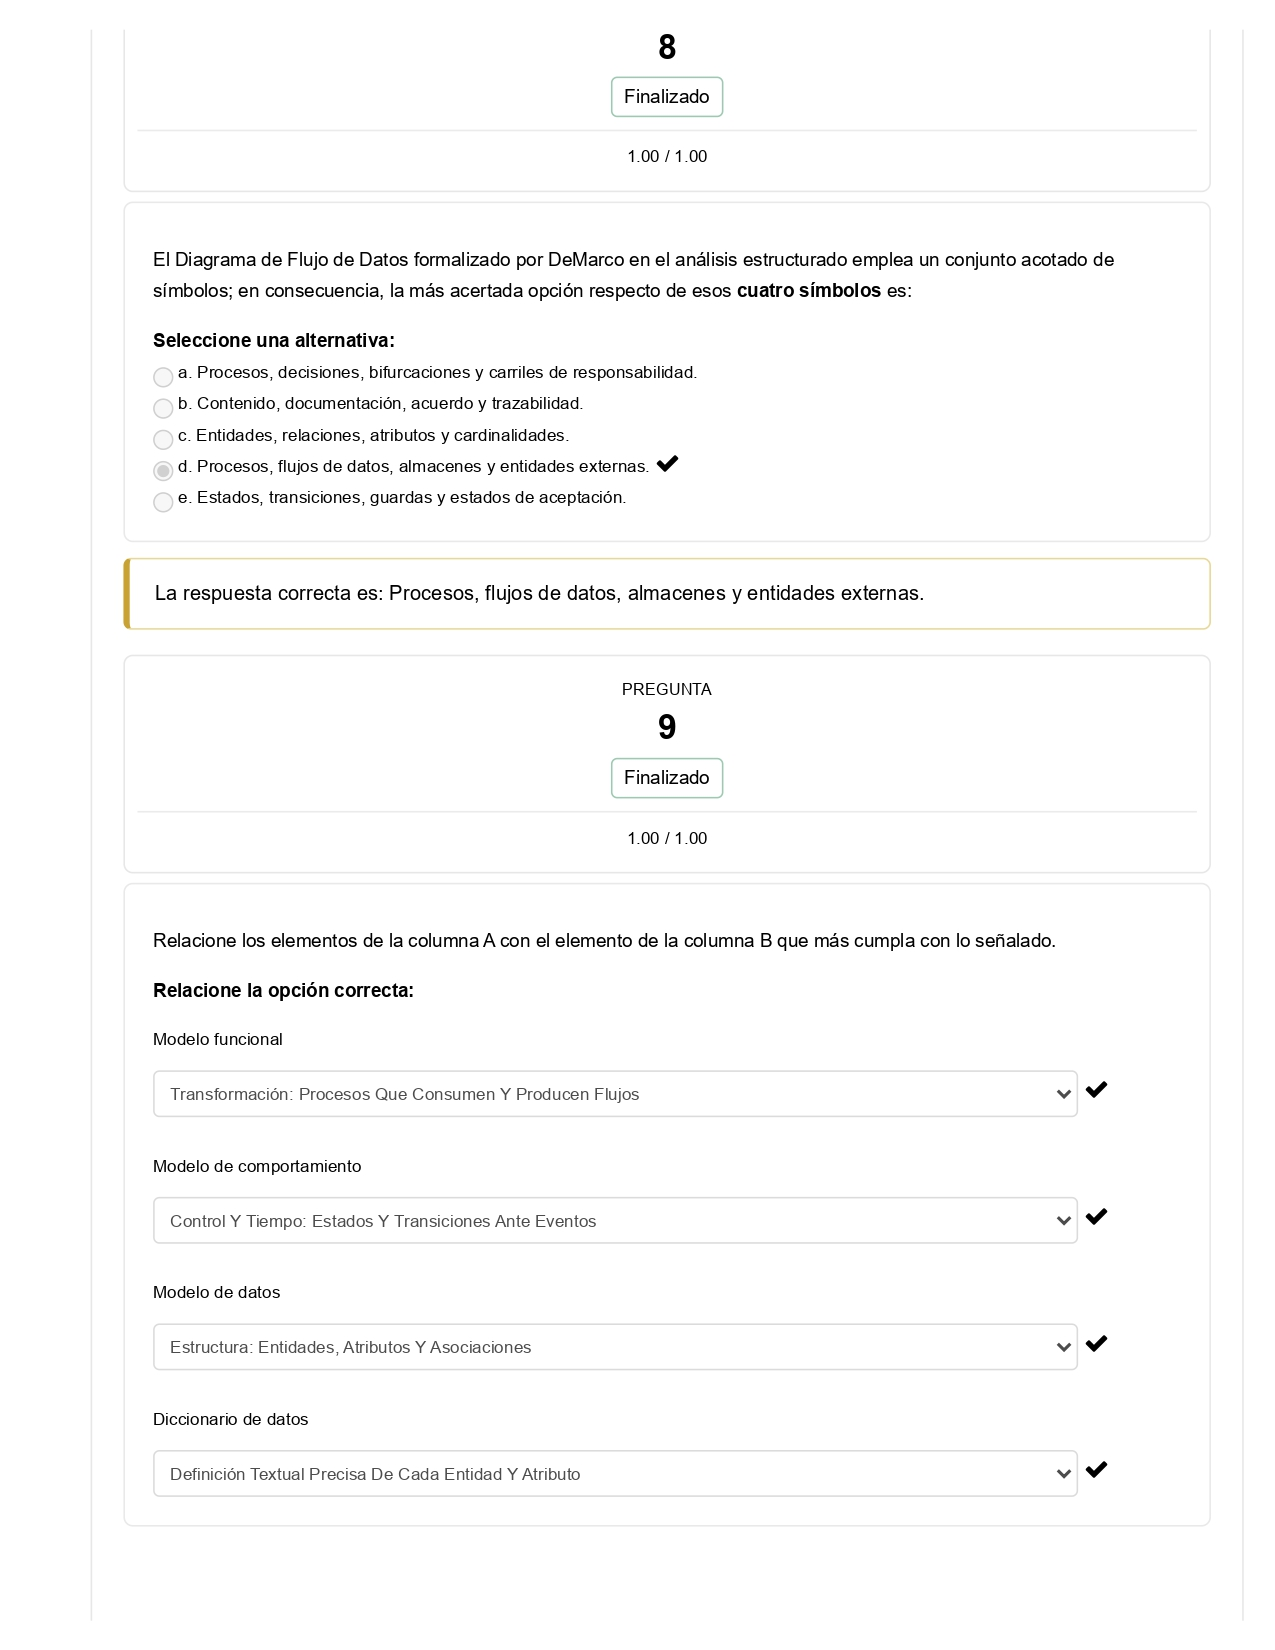
\includegraphics[width=\paperwidth,height=\paperheight,keepaspectratio]{figuras/revision_pg-5.jpg}\par
	\newpage
	\thispagestyle{empty}
	\noindent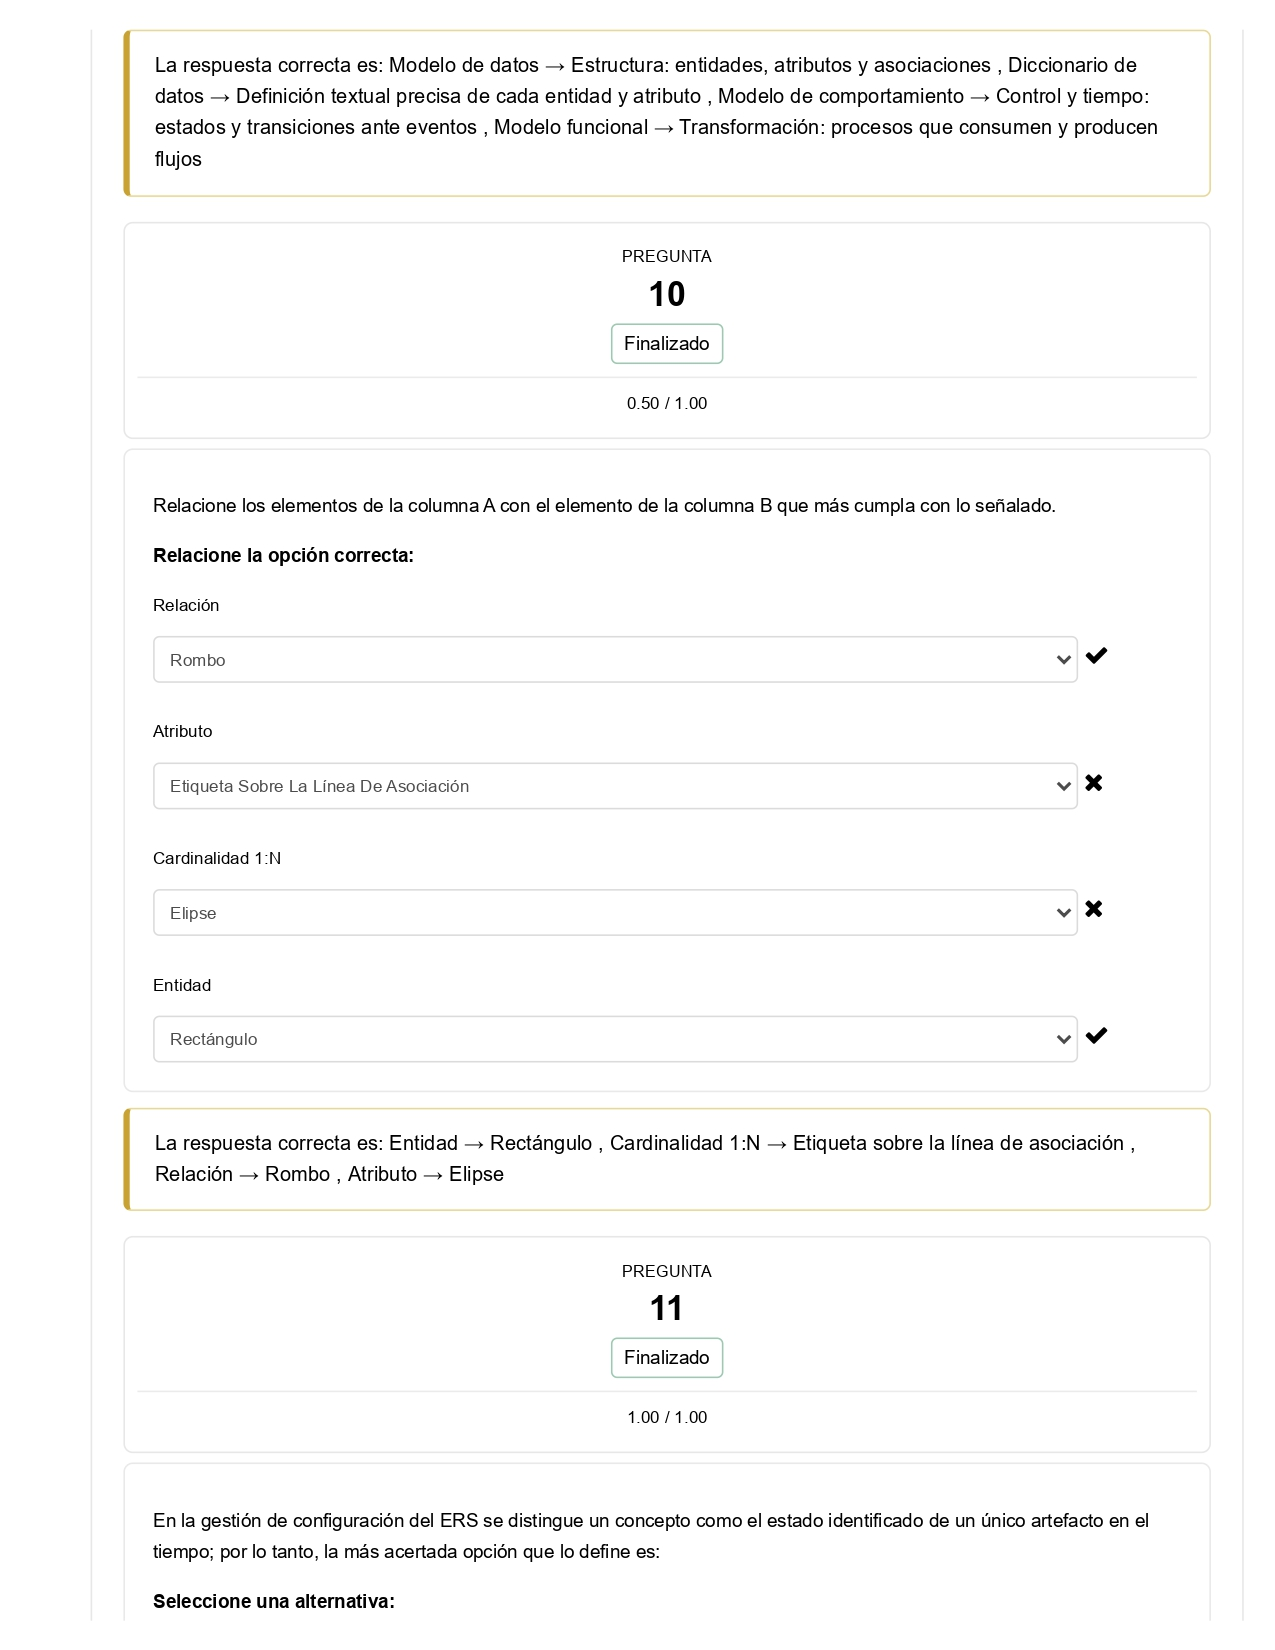
\includegraphics[width=\paperwidth,height=\paperheight,keepaspectratio]{figuras/revision_pg-6.jpg}\par
	\newpage
	\thispagestyle{empty}
	\noindent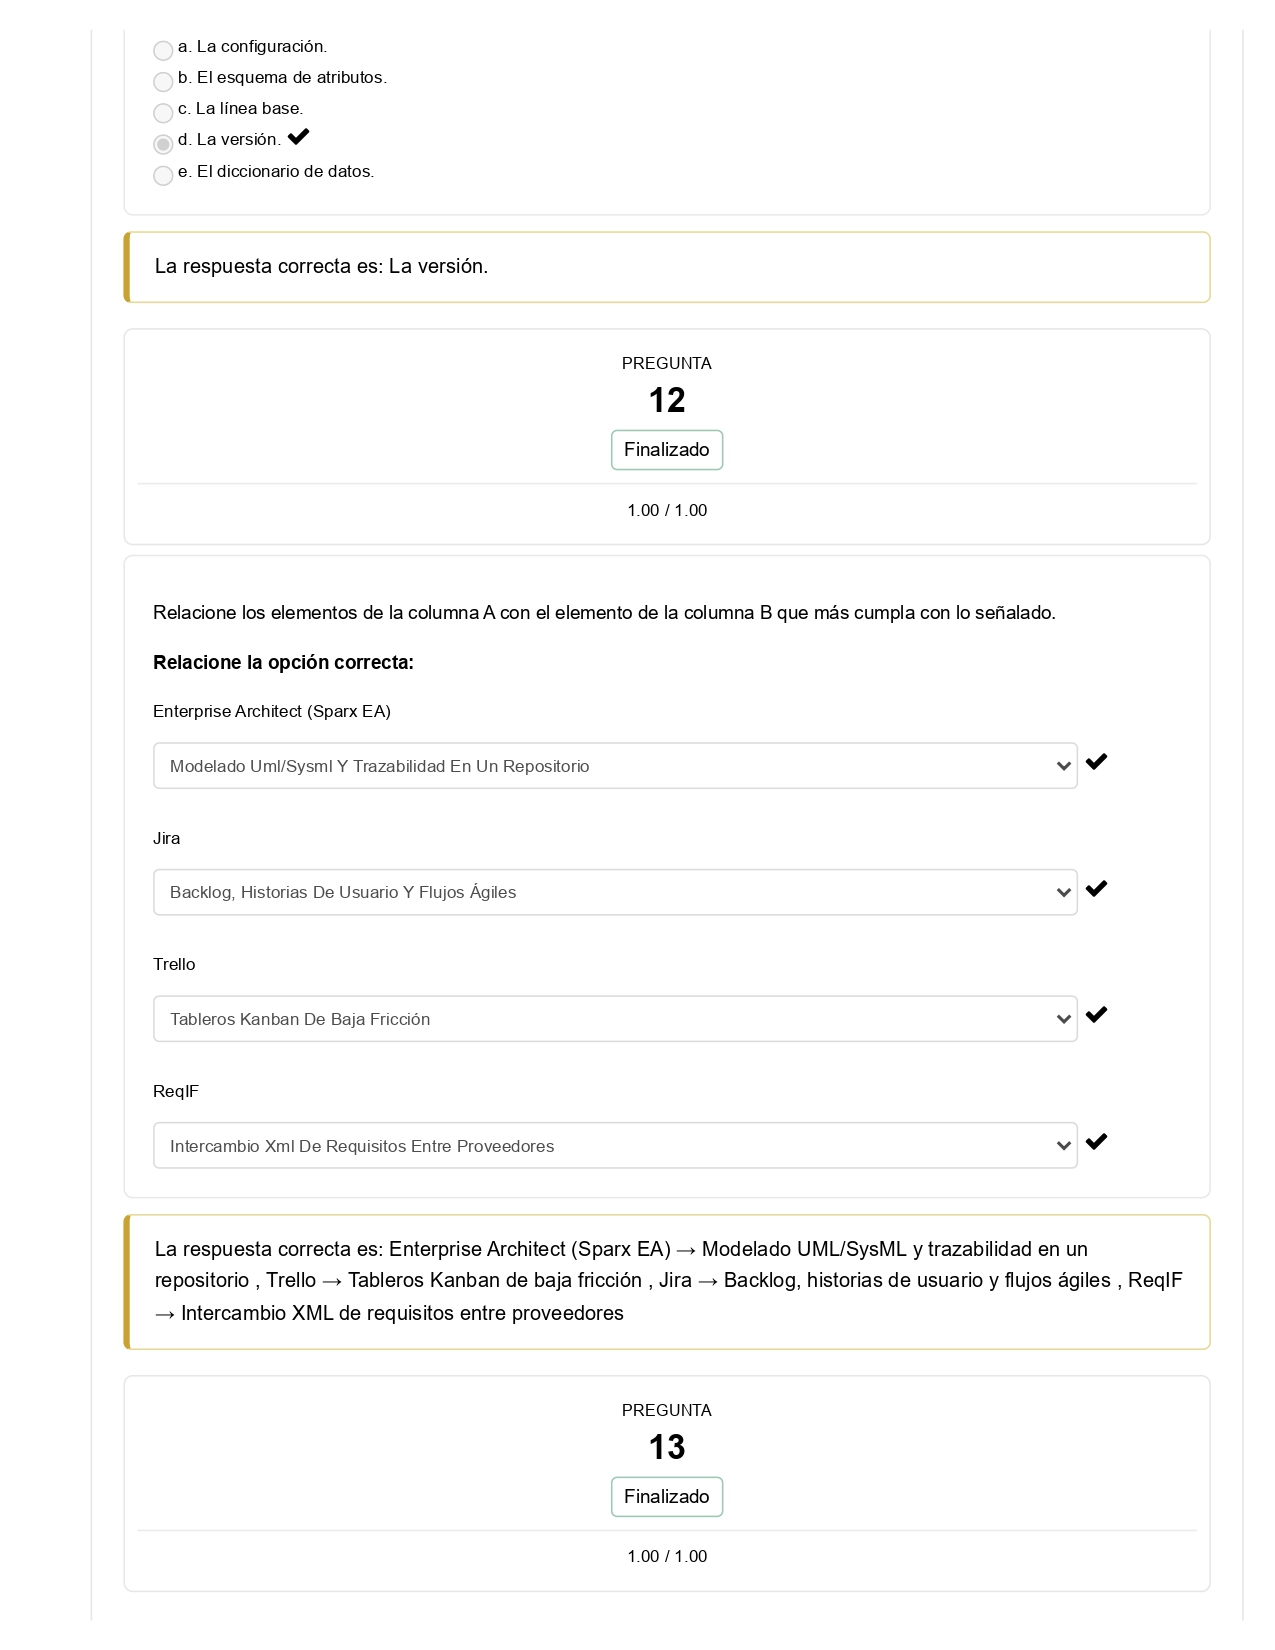
\includegraphics[width=\paperwidth,height=\paperheight,keepaspectratio]{figuras/revision_pg-7.jpg}\par
	\newpage
	\thispagestyle{empty}
	\noindent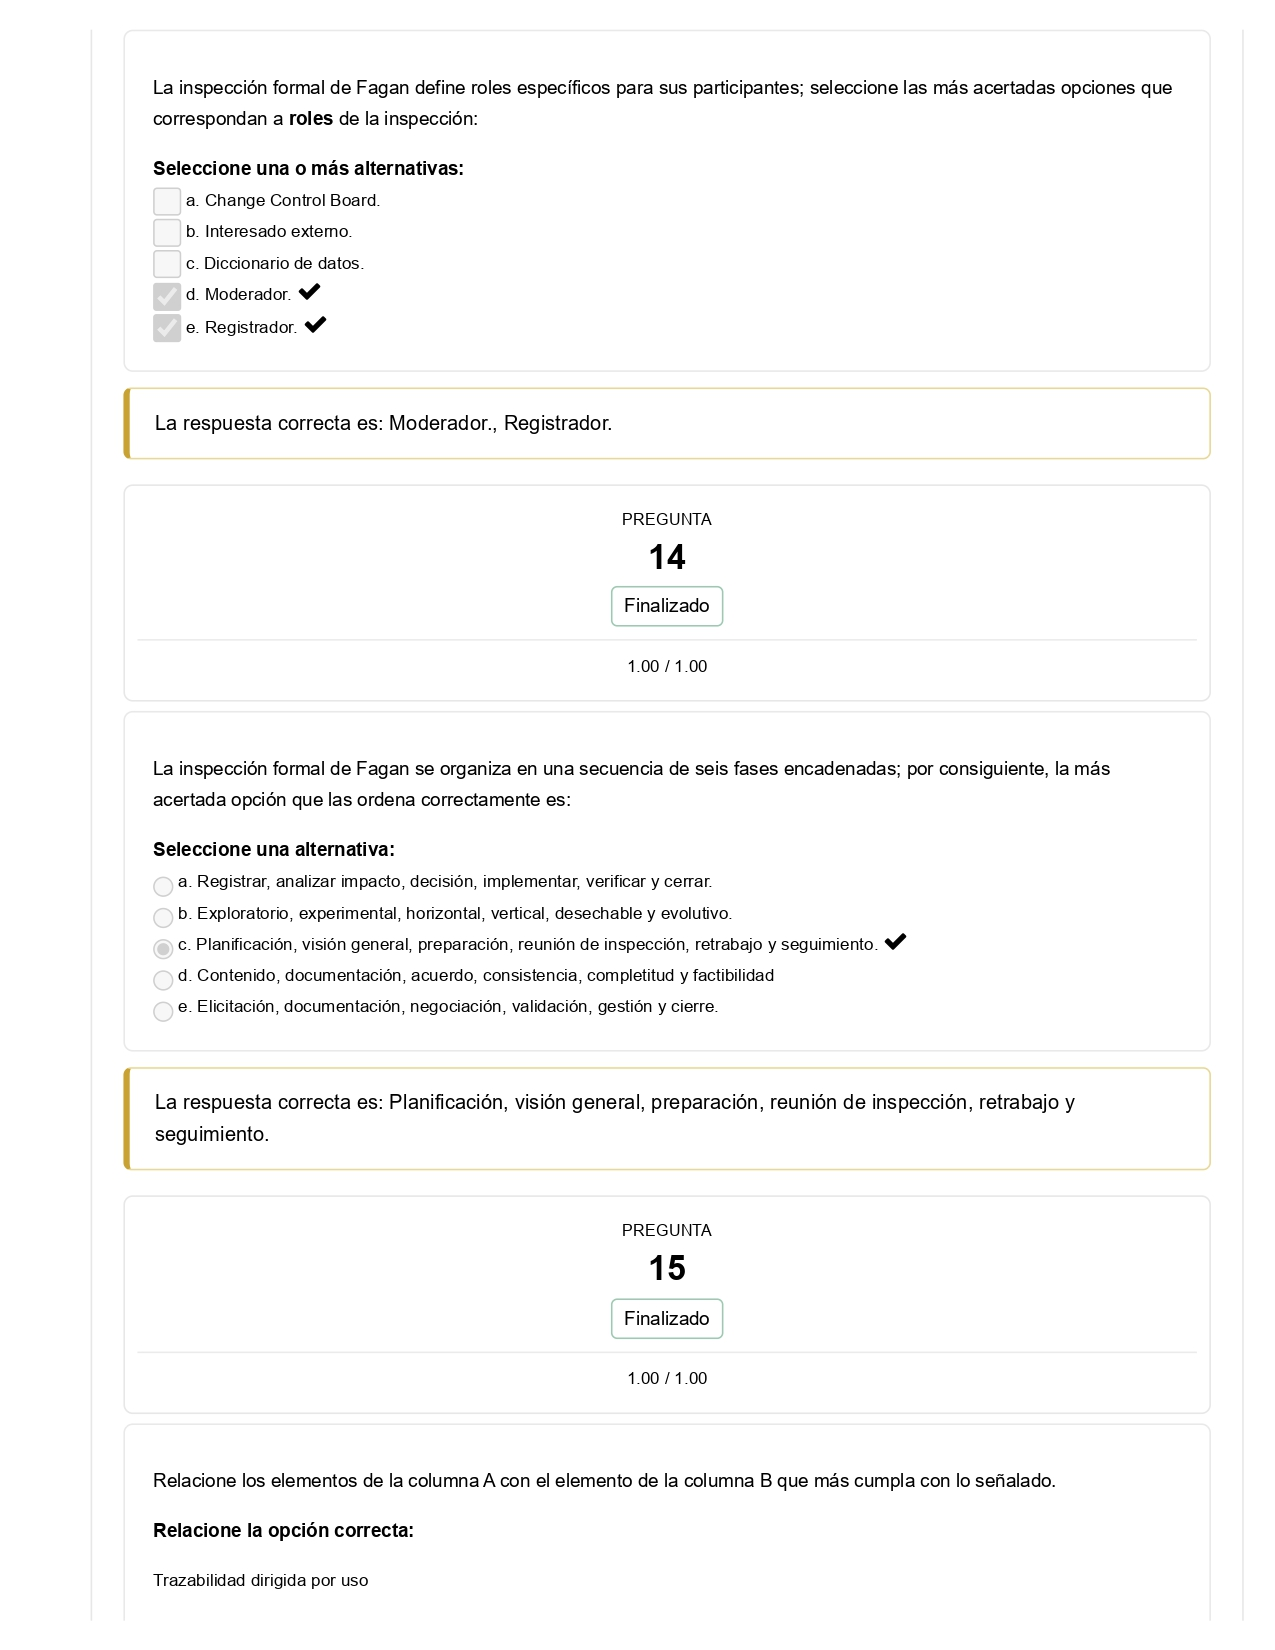
\includegraphics[width=\paperwidth,height=\paperheight,keepaspectratio]{figuras/revision_pg-8.jpg}\par
	\newpage
	\thispagestyle{empty}
	\noindent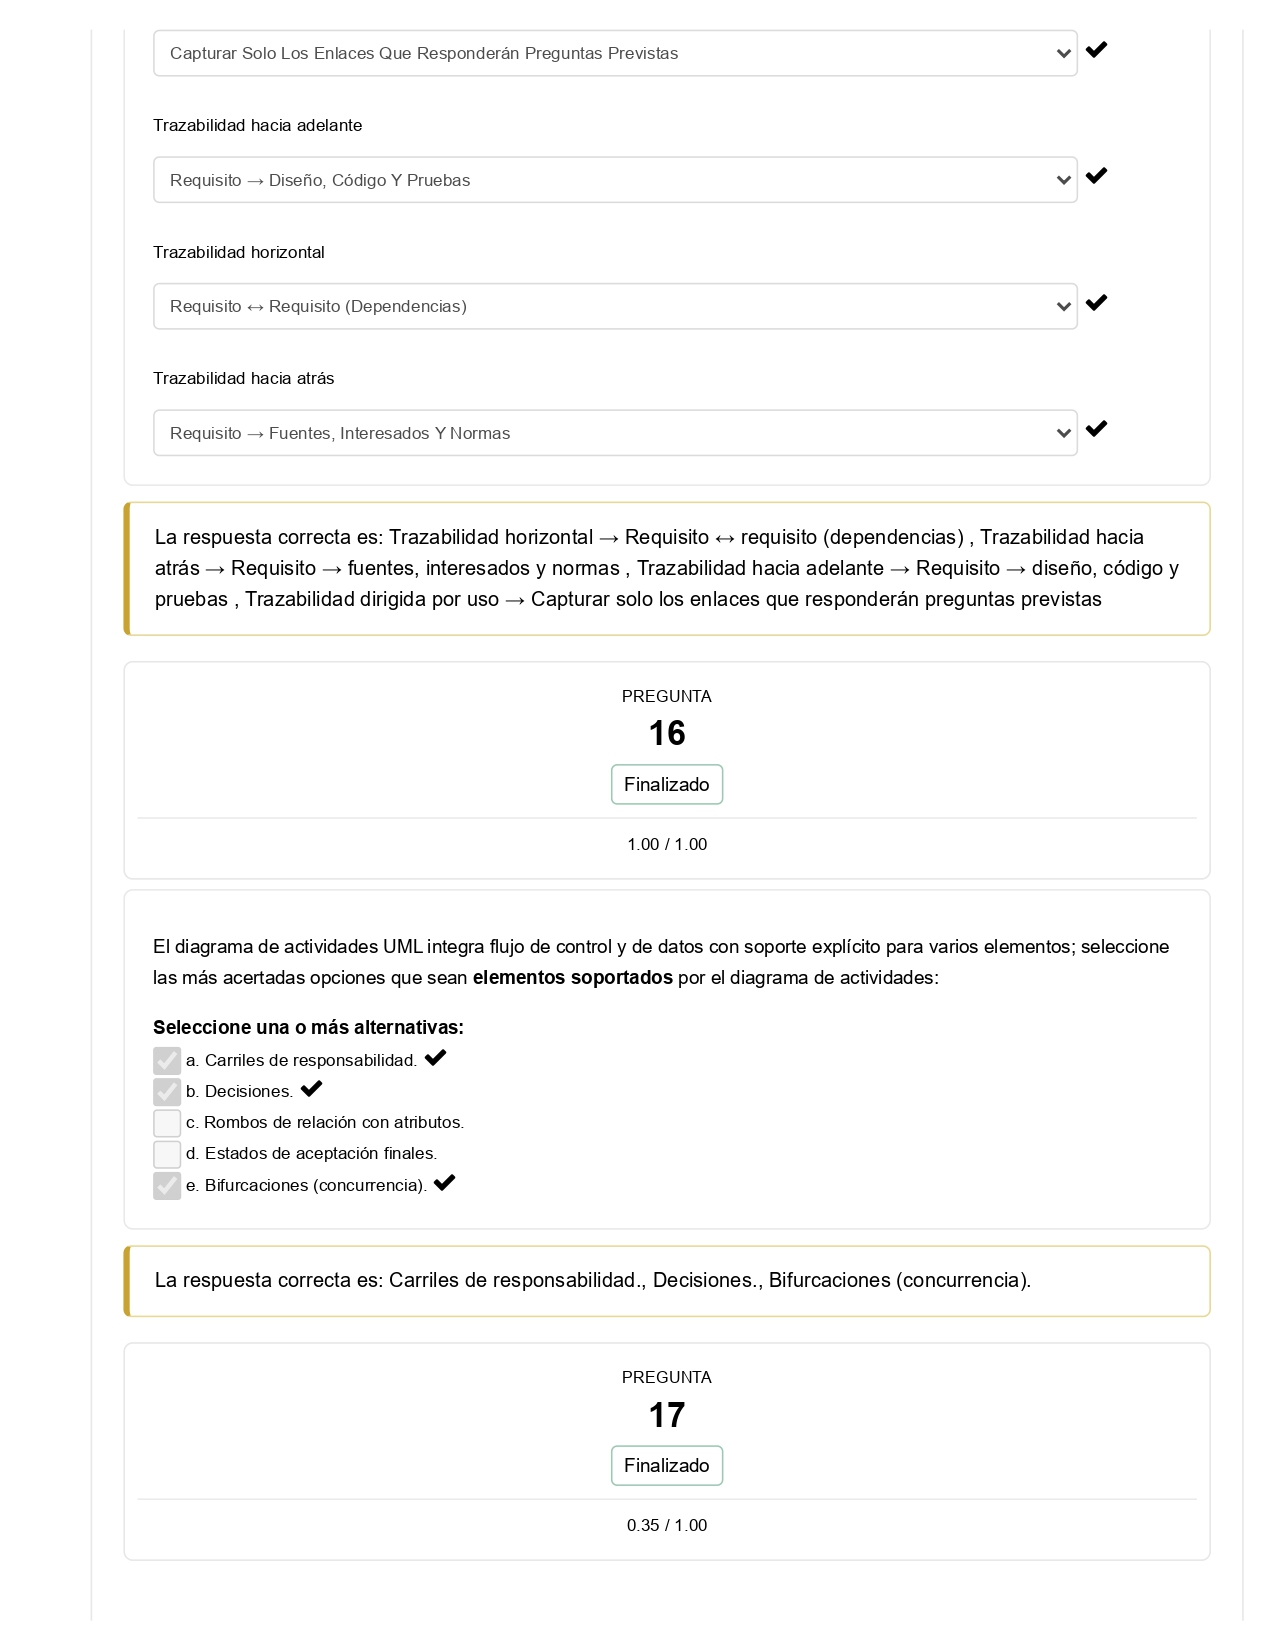
\includegraphics[width=\paperwidth,height=\paperheight,keepaspectratio]{figuras/revision_pg-9.jpg}\par
	\newpage
	\thispagestyle{empty}
	\noindent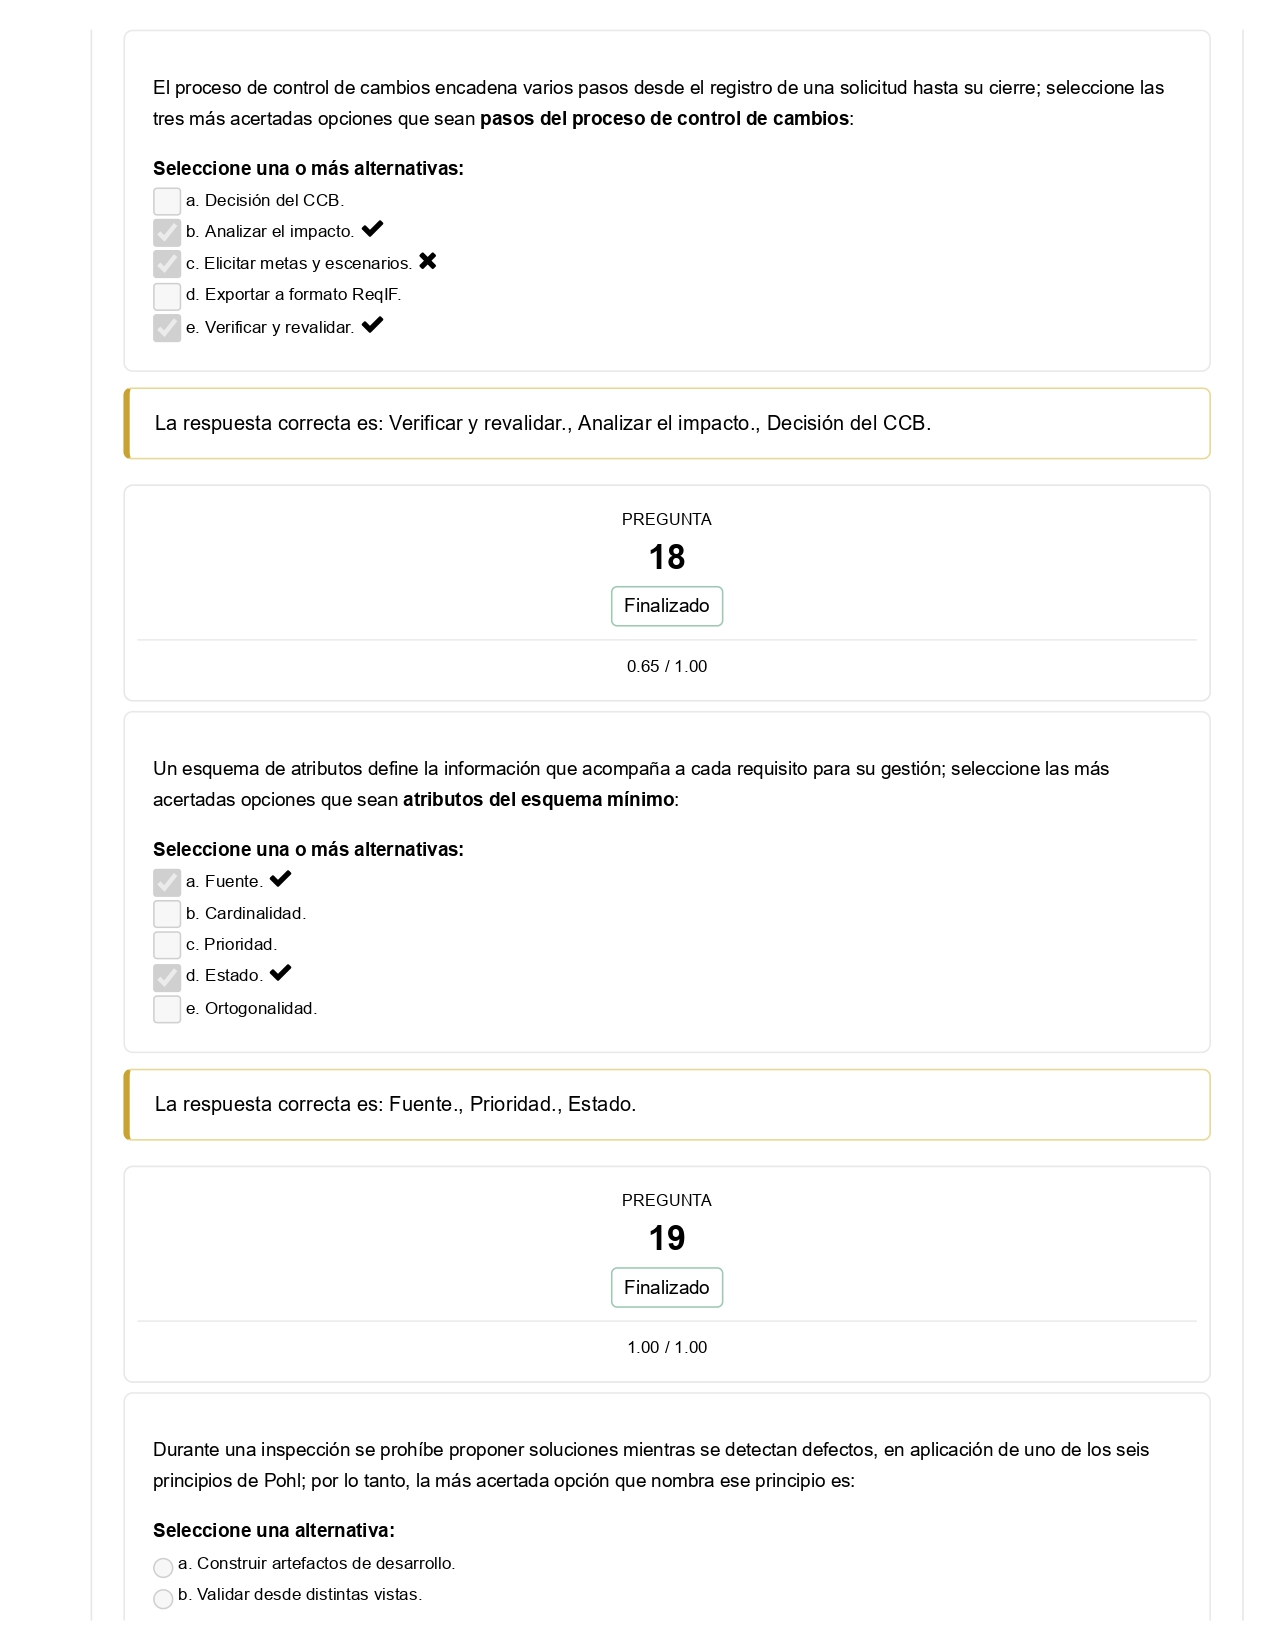
\includegraphics[width=\paperwidth,height=\paperheight,keepaspectratio]{figuras/revision_pg-10.jpg}\par
	\newpage
	\thispagestyle{empty}
	\noindent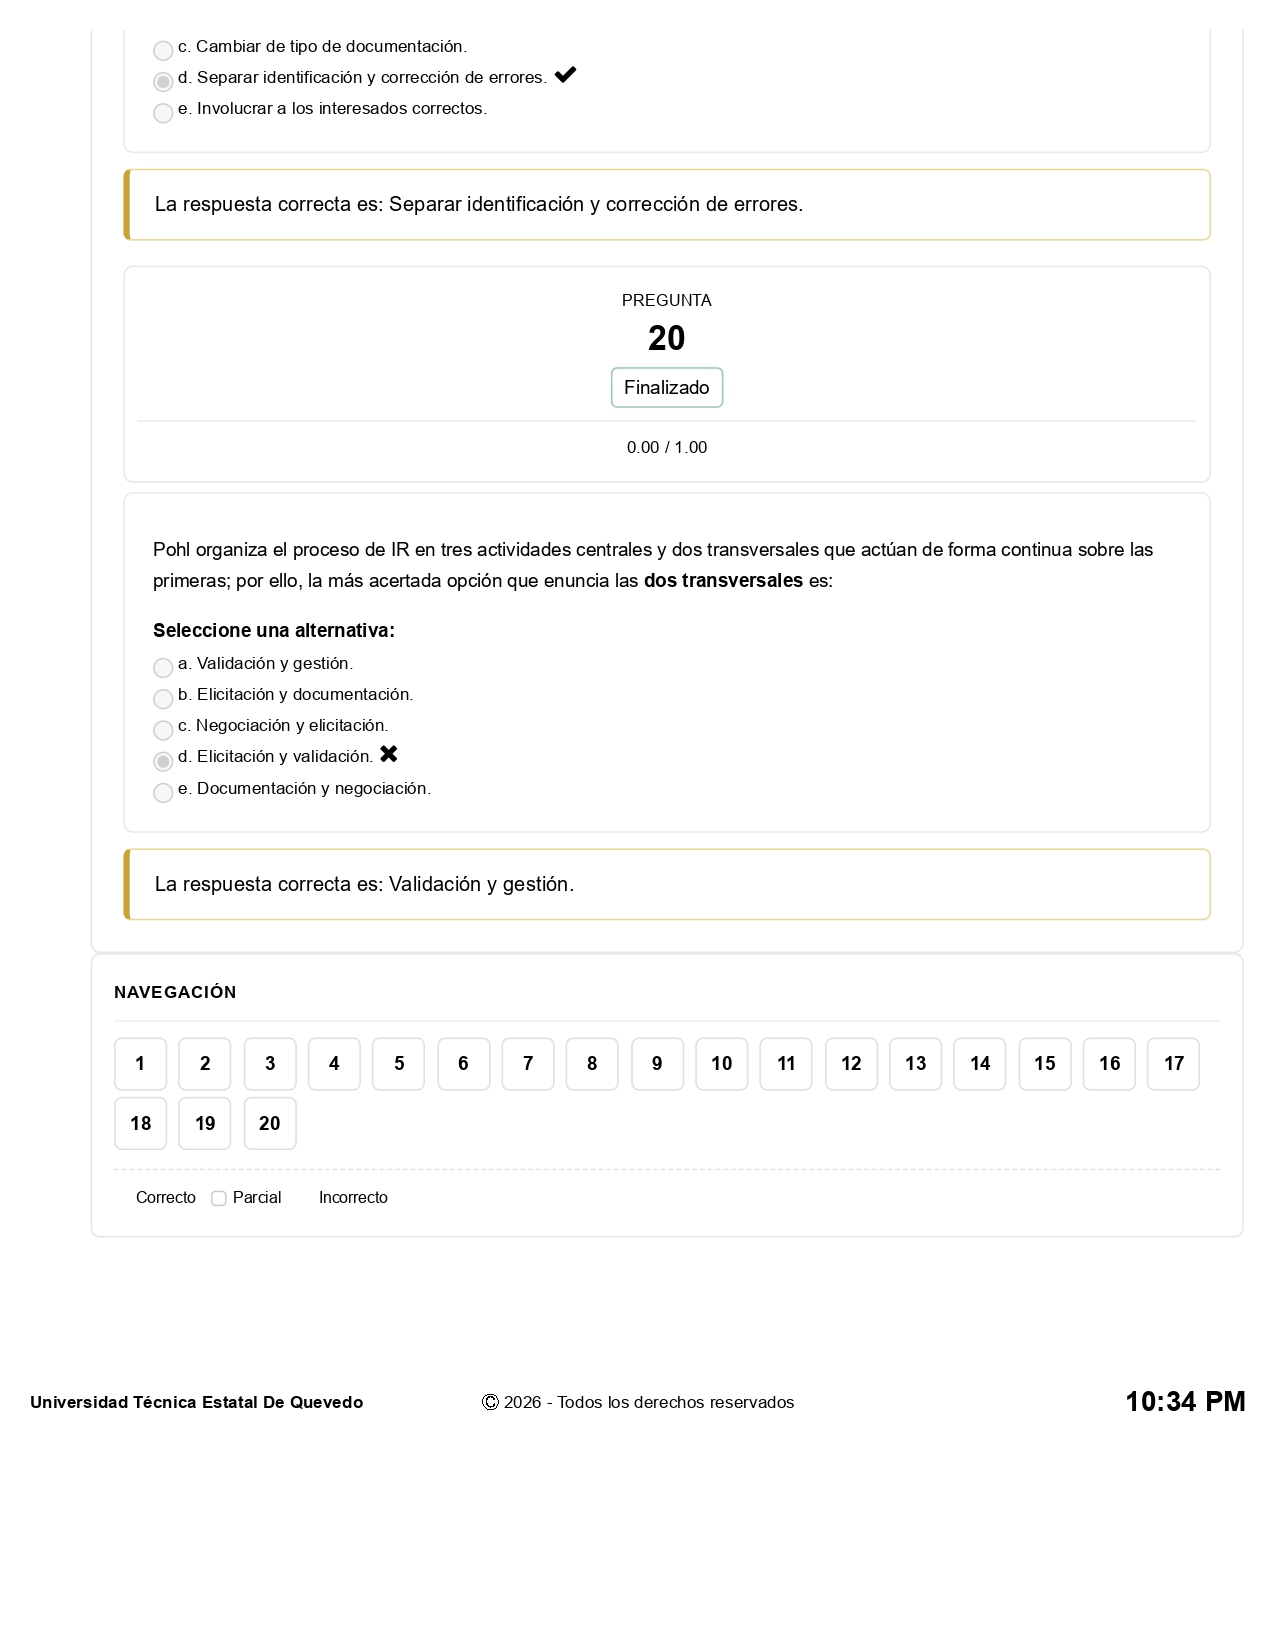
\includegraphics[width=\paperwidth,height=\paperheight,keepaspectratio]{figuras/revision_pg-11.jpg}\par
	\restoregeometry
	
\end{document}